% SIAM Article Template
\documentclass[review,onefignum,onetabnum]{siamonline171218}

% Information that is shared between the article and the supplement
% (title and author information, macros, packages, etc.) goes into
% ex_shared.tex. If there is no supplement, this file can be included
% directly.

% SIAM Shared Information Template
% This is information that is shared between the main document and any
% supplement. If no supplement is required, then this information can
% be included directly in the main document.


% Packages and macros go here
\usepackage{lipsum}
\usepackage{amsfonts}
\usepackage{graphicx}
\usepackage{epstopdf}
\usepackage{soul}
\usepackage{caption}
\usepackage{subcaption}
\usepackage{algorithm}
\usepackage{algpseudocode}
\usepackage{enumitem}
\usepackage{comment}
\ifpdf
  \DeclareGraphicsExtensions{.eps,.pdf,.png,.jpg}
\else
  \DeclareGraphicsExtensions{.eps}
\fi

% \usepackage[dvipsnames,x11names]{xcolor}

\usepackage{booktabs}
\usepackage{multirow}
\usepackage{annotate-equations}

% Prevent itemized lists from running into the left margin inside theorems and proofs
\usepackage{enumitem}
\setlist[enumerate]{leftmargin=.5in}
\setlist[itemize]{leftmargin=.5in}

% Add a serial/Oxford comma by default.
\newcommand{\creflastconjunction}{, and~}

% Used for creating new theorem and remark environments
\newsiamremark{remark}{Remark}
\newsiamremark{hypothesis}{Hypothesis}
\crefname{hypothesis}{Hypothesis}{Hypotheses}
\newsiamthm{claim}{Claim}

% Sets running headers as well as PDF title and authors
% \headers{Utilizing Covariance Uncertainty in Multi-fidelity Estimation with Approximate Control Variates}{T. Coons, A. Jivani, and X. Huan}

\headers{Multifidelity SVGD}{A. Jivani, T. Coons and X. Huan}

% Title. If the supplement option is on, then "Supplementary Material"
% is automatically inserted before the title.
% \title{Utilizing Covariance Uncertainty in Multi-fidelity Estimation with Approximate Control Variates\thanks{Submitted to the editors DATE.
% \funding{Enter funding sources!}}}
\title{Scalable Stein Variational Gradient Descent via Multifidelity Particle Transport with Application to Bayesian Inference\thanks{Submitted to the editors DATE.
\funding{This work is supported in part by the National Science Foundation Graduate Research Fellowship under Grant No. DGE 1841052, the Department of Navy award N00014-23-1-2735 issued by the Office of Naval Research, and through computational resources and services provided by Advanced Research Computing at the University of Michigan, Ann Arbor.}}}

% Authors: full names plus addresses.
\author{Aniket Jivani\thanks{Department of Mechanical Engineering, University of Michigan, Ann Arbor, MI 48109 
  (\email{ajivani@umich.edu}, \url{https://me.engin.umich.edu/}).}
\and Thomas E. Coons\footnotemark[2]
\and Xun Huan\footnotemark[2]}

\usepackage{amsopn}
\DeclareMathOperator{\diag}{diag}


%%%% HELPER CODE FOR DEALING WITH EXTERNAL REFERENCES ON OVERLEAF
% (from an answer by cyberSingularity at http://tex.stackexchange.com/a/69832/226)
%%%
\makeatletter
\newcommand*{\addFileDependency}[1]{% argument=file name and extension
  \typeout{(#1)}% latexmk will find this if $recorder=0 (however, in that case, it will ignore #1 if it is a .aux or .pdf file etc and it exists! if it doesn't exist, it will appear in the list of dependents regardless)
  \@addtofilelist{#1}% if you want it to appear in \listfiles, not really necessary and latexmk doesn't use this
  \IfFileExists{#1}{}{\typeout{No file #1.}}% latexmk will find this message if #1 doesn't exist (yet)
}
\makeatother

\newcommand*{\myexternaldocument}[1]{%
    \externaldocument{#1}%
    \addFileDependency{#1.tex}%
    \addFileDependency{#1.aux}%
}
%%% END HELPER CODE

%%% Local Variables: 
%%% mode:latex
%%% TeX-master: "ex_article"
%%% End: 



% % SIAM Shared Information Template
% % This is information that is shared between the main document and any
% % supplement. If no supplement is required, then this information can
% % be included directly in the main document.


% % Packages and macros go here
% \usepackage{lipsum}
% \usepackage{amsfonts}
% \usepackage{graphicx}
% \usepackage{epstopdf}
% \usepackage{algorithmic}
% \ifpdf
%   \DeclareGraphicsExtensions{.eps,.pdf,.png,.jpg}
% \else
%   \DeclareGraphicsExtensions{.eps}
% \fi

% % Prevent itemized lists from running into the left margin inside theorems and proofs
% \usepackage{enumitem}
% \setlist[enumerate]{leftmargin=.5in}
% \setlist[itemize]{leftmargin=.5in}

% % Add a serial/Oxford comma by default.
% \newcommand{\creflastconjunction}{, and~}

% % Used for creating new theorem and remark environments
% \newsiamremark{remark}{Remark}
% \newsiamremark{hypothesis}{Hypothesis}
% \crefname{hypothesis}{Hypothesis}{Hypotheses}
% \newsiamthm{claim}{Claim}

% % Sets running headers as well as PDF title and authors
% \headers{Multi-fidelity SVGD}{A. Jivani, T. Coons, X. Huan}

% % Title. If the supplement option is on, then "Supplementary Material"
% % is automatically inserted before the title.
% % \title{An Example Article\thanks{Submitted to the editors DATE.
% % \funding{This work was funded by the Fog Research Institute under contract no.~FRI-454.}}}

% \title{Scalable Stein Variational Gradient Descent via Multifidelity Particle Transport with Application to Bayesian Inference\thanks{Submitted to the editors DATE.
% \funding{This work is supported in part by the National Science Foundation Graduate Research Fellowship under Grant No. DGE 1841052, the Department of Navy award N00014-23-1-2735 issued by the Office of Naval Research, and through computational resources and services provided by Advanced Research Computing at the University of Michigan, Ann Arbor.}}}

% % Authors: full names plus addresses.
% \author{Aniket Jivani \thanks{Department of Mechanical Engineering, University of Michigan, Ann Arbor, MI, 48109 
%   (Correspondence: \email{ajivani@umich.edu}).}
% \and Thomas E. Coons \footnotemark[2]
% \and Xun Huan \footnotemark[2]}

% \usepackage{amsopn}
% \DeclareMathOperator{\diag}{diag}


% %%%% HELPER CODE FOR DEALING WITH EXTERNAL REFERENCES ON OVERLEAF
% % (from an answer by cyberSingularity at http://tex.stackexchange.com/a/69832/226)
% %%%
% \makeatletter
% \newcommand*{\addFileDependency}[1]{% argument=file name and extension
%   \typeout{(#1)}% latexmk will find this if $recorder=0 (however, in that case, it will ignore #1 if it is a .aux or .pdf file etc and it exists! if it doesn't exist, it will appear in the list of dependents regardless)
%   \@addtofilelist{#1}% if you want it to appear in \listfiles, not really necessary and latexmk doesn't use this
%   \IfFileExists{#1}{}{\typeout{No file #1.}}% latexmk will find this message if #1 doesn't exist (yet)
% }
% \makeatother

% \newcommand*{\myexternaldocument}[1]{%
%     \externaldocument{#1}%
%     \addFileDependency{#1.tex}%
%     \addFileDependency{#1.aux}%
% }
% %%% END HELPER CODE

% %%% Local Variables: 
% %%% mode:latex
% %%% TeX-master: "ex_article"
% %%% End: 


% Optional PDF information
\ifpdf
\hypersetup{
  pdftitle={An Example Article},
  pdfauthor={D. Doe, P. T. Frank, and J. E. Smith}
}
\fi

% The next statement enables references to information in the
% supplement. See the xr-hyperref package for details.

%% Use \myexternaldocument on Overleaf
% \myexternaldocument{ex_supplement}

% FundRef data to be entered by SIAM
%<funding-group>
%<award-group>
%<funding-source>
%<named-content content-type="funder-name"> 
%</named-content> 
%<named-content content-type="funder-identifier"> 
%</named-content>
%</funding-source>
%<award-id> </award-id>
%</award-group>
%</funding-group>

% \documentclass[12pt]{article}
% \usepackage{graphicx} % Required for inserting images
% \usepackage[utf8]{inputenc}

\usepackage{hyperref}
\usepackage{xcolor}

\hypersetup{
  colorlinks=true,
  citecolor=blue,
  linkcolor=red,
  urlcolor=magenta,
  }
  % citebordercolor=false}

\usepackage{float}
\usepackage{url}
\usepackage{tabularx}
% \usepackage{amsmath}
% \usepackage{amsfonts}
\usepackage{amssymb}
\usepackage{mathtools}
\usepackage{xurl}
\usepackage{lineno}
% \usepackage{amsthm}
\usepackage{epsfig}
% \usepackage[linesnumbered, ruled]{algorithm2e}

\usepackage{ulem}
\newcommand{\stkout}[1]{\ifmmode\text{\sout{\ensuremath{#1}}}\else\sout{#1}\fi}
\usepackage{multirow}
\usepackage{longtable}
\setlength\LTleft{0pt}
\usepackage{tabularx}
% \setlength\LTleft{0pt}
% \bibliographystyle{unsrt}
% \bibliographystyle{agu}
% \bibliographystyle{plainnat}
\usepackage{epsfig}
% \usepackage[linesnumbered, ruled]{algorithm2e}
\usepackage{natbib}
% \usepackage{color}
%
% \clearpage{}%

\newcommand\prob{\mathbb{P}}

\newcommand{\xh}[1]{\textcolor{orange}{\textbf{(xh:)} #1}}
\newcommand{\tc}[1]{\textcolor{red}{\textbf{(tc:)} #1}}
\newcommand{\aj}[1]{\textcolor{magenta}{\textbf{(aj:)} #1}}

%
\newcommand{\resp}[1]{\textcolor{red}{\textbf{Response: } #1}}
\newcommand{\respc}[1]{\textcolor{red}{#1}}

\newcommand\Myperm[2][^n]{\prescript{#1\mkern-2.5mu}{}P_{#2}}
\newcommand\Mycomb[2][^n]{\prescript{#1\mkern-0.5mu}{}C_{#2}}
%
\renewcommand{\[}{\left[}
\renewcommand{\]}{\right]}
\renewcommand{\(}{\left(}
\renewcommand{\)}{\right)}

%
\newcommand{\dd}[2]{\frac{d #1}{d #2}}
\newcommand{\ddt}[1]{\frac{d #1}{d t}}
\newcommand{\ddd}[2]{\frac{d^2 #1}{d #2^2}}
\newcommand{\dddt}[1]{\frac{d^2 #1}{d t^2}}
\newcommand{\pp}[2]{\frac{\partial #1}{\partial #2}}
\newcommand{\ppp}[2]{\frac{\partial^2 #1}{\partial #2^2}}
\newcommand{\pppp}[2]{\frac{\partial^3 #1}{\partial #2^3}}
\newcommand{\ppppp}[2]{\frac{\partial^4 #1}{\partial #2^4}}

\newcommand{\adj}[1]{#1^{*}}
\newcommand{\abs}[1]{\left|#1\right|}
\newcommand{\divergence}[1]{\nabla \cdot #1}
\newcommand{\enorm}[1]{\vvvert #1 \vvvert}
\newcommand{\grad}[1]{\nabla #1}
\newcommand{\laplace}[1]{\nabla^2 #1}
\newcommand{\norm}[2]{\left\|\, #1 \,\right\|_{#2}}
\newcommand{\order}[1]{\mathcal{O}\(#1\)}
\newcommand{\supp}{\mathop{\mathrm{supp}}}
\newcommand{\vvvert}{|\kern-1pt|\kern-1pt|}

\newcommand{\eq}[1]{\mathop{\,{\buildrel #1 \over =}\,}}
\newcommand{\ap}[1]{\mathop{\,{\buildrel #1 \over \approx}\,}}

%

%
\newcommand{\hg}{\hat{g}}
\newcommand{\hh}{\hat{h}}
\newcommand{\hi}{\hat{i}}
\newcommand{\hj}{\hat{j}}
\newcommand{\hk}{\hat{k}}
\newcommand{\hm}{\hat{m}}
\newcommand{\hn}{\hat{n}}
\newcommand{\hs}{\hat{s}}
\newcommand{\hu}{\hat{u}}
\newcommand{\hv}{\hat{v}}
\newcommand{\hx}{\hat{x}}

\newcommand{\hA}{\hat{A}}
\newcommand{\hC}{\hat{C}}
\newcommand{\hI}{\hat{I}}
\newcommand{\hJ}{\hat{J}}
\newcommand{\hN}{\hat{N}}
\newcommand{\hT}{\hat{T}}
\newcommand{\hU}{\hat{U}}

\newcommand{\hbf}{\boldsymbol{\hat{f}}}
\newcommand{\hbg}{\boldsymbol{\hat{g}}}
\newcommand{\hsig}{\hat{\sigma}}

%
\newcommand{\barg}{\bar{g}}
\newcommand{\barh}{\bar{h}}
\newcommand{\barm}{\bar{m}}
\newcommand{\barv}{\bar{v}}
\newcommand{\barw}{\bar{w}}
\newcommand{\barx}{\bar{x}}
\newcommand{\bary}{\bar{y}}

\newcommand{\barB}{\bar{B}}
\newcommand{\barC}{\bar{C}}
\newcommand{\barH}{\bar{H}}
\newcommand{\barJ}{\bar{J}}
\newcommand{\barN}{\bar{N}}
\newcommand{\barR}{\bar{R}}

\newcommand{\barmu}{\bar{\mu}}

%
\newcommand{\tf}{\tilde{f}}
\newcommand{\thh}{\tilde{h}}

\newcommand{\tA}{\tilde{A}}
\newcommand{\tg}{\tilde{g}}
\newcommand{\tH}{\tilde{H}}
\newcommand{\tJ}{\tilde{J}}
\newcommand{\tQ}{\tilde{Q}}
\newcommand{\tT}{\tilde{T}}

\newcommand{\tmu}{\tilde{\mu}}
\newcommand{\ttheta}{\tilde{\theta}}
\newcommand{\txi}{\tilde{\xi}}

\newcommand{\tTheta}{\tilde{\Theta}}
\newcommand{\tXi}{\tilde{\Xi}}

%
\newcommand{\mb}[1]{\mathbf{#1}}
\newcommand{\sbf}[1]{\boldsymbol{#1}}

\newcommand{\bb}{\textbf{b}}
\newcommand{\bd}{\textbf{d}}
\newcommand{\bee}{\textbf{e}}
\newcommand{\bff}{\textbf{f}}
\newcommand{\bh}{\textbf{h}}
\newcommand{\bg}{\textbf{g}}
\newcommand{\bk}{\textbf{k}}
\newcommand{\bii}{\textbf{i}}
\newcommand{\bj}{\textbf{j}}
\newcommand{\bl}{\textbf{l}}
\newcommand{\bn}{\textbf{n}}
\newcommand{\bp}{\textbf{p}}
\newcommand{\br}{\textbf{r}}
\newcommand{\bs}{\textbf{s}}
\newcommand{\bt}{\textbf{t}}
\newcommand{\bu}{\textbf{u}}
\newcommand{\bv}{\textbf{v}}
\newcommand{\bw}{\textbf{w}}
\newcommand{\bx}{\textbf{x}}
\newcommand{\by}{\textbf{y}}

\newcommand{\bA}{\mathbf{A}}
\newcommand{\bC}{\mathbf{C}}
\newcommand{\bE}{\mathbf{E}}
\newcommand{\bF}{\mathbf{F}}
\newcommand{\bG}{\mathbf{G}}
\newcommand{\bI}{\mathbf{I}}
\newcommand{\bK}{\mathbf{K}}
\newcommand{\bN}{\mathbf{N}}
\newcommand{\bQ}{\mathbf{Q}}
\newcommand{\bR}{\mathbf{R}}
\newcommand{\bT}{\mathbf{T}}
\newcommand{\bU}{\mathbf{U}}
\newcommand{\bV}{\mathbf{V}}
\newcommand{\bY}{\mathbf{Y}}

\newcommand{\balpha}{\boldsymbol{\alpha}}
\newcommand{\bbeta}{\boldsymbol{\beta}}
\newcommand{\bepsilon}{\boldsymbol{\epsilon}}
\newcommand{\bhsig}{\boldsymbol{\hsig}}
\newcommand{\bpsi}{\boldsymbol{\psi}}
\newcommand{\bsig}{\boldsymbol{\sigma}}
\newcommand{\btau}{\boldsymbol{\tau}}
\newcommand{\bmu}{\boldsymbol{\mu}}
\newcommand{\btheta}{\boldsymbol{\theta}}
\newcommand{\bphi}{\boldsymbol{\phi}}
\newcommand{\bxi}{\boldsymbol{\xi}}

\newcommand{\bDelta}{\boldsymbol{\Delta}}
\newcommand{\bTheta}{\boldsymbol{\Theta}}
\newcommand{\bXi}{\boldsymbol{\Xi}}
\newcommand{\bOmega}{\boldsymbol{\Omega}}
\newcommand{\bSigma}{\boldsymbol{\Sigma}}

%
\newcommand{\EE}{\mathbb{E}}
\newcommand{\II}{\mathbb{I}}
\newcommand{\NN}{\mathbb{N}}
\newcommand{\QQ}{\mathbb{Q}}
\newcommand{\PP}{\mathbb{P}}
\newcommand{\RR}{\mathbb{R}}

%
\newcommand{\vt}{\vec{t}}
\newcommand{\vu}{\vec{u}}
\newcommand{\vv}{\vec{v}}
\newcommand{\vx}{\vec{x}}

\newcommand{\vV}{\vec{V}}

\newcommand{\vo}{\vec{\omega}}

%
\newcommand{\dotk}{\dot{k}}
\newcommand{\dotm}{\dot{m}}
\newcommand{\dotx}{\dot{x}}

\newcommand{\dotomega}{\dot{\omega}}

%
\newcommand{\CA}{\mathcal{A}}
\newcommand{\CB}{\mathcal{B}}
\newcommand{\CD}{\mathcal{D}}
\newcommand{\CE}{\mathcal{E}}
\newcommand{\CF}{\mathcal{F}}
\newcommand{\CG}{\mathcal{G}}
\newcommand{\CH}{\mathcal{H}}
\newcommand{\CJ}{\mathcal{J}}
\newcommand{\CK}{\mathcal{K}}
\newcommand{\CL}{\mathcal{L}}
\newcommand{\CM}{\mathcal{M}}
\newcommand{\CN}{\mathcal{N}}
\newcommand{\CQ}{\mathcal{N}}
\newcommand{\CR}{\mathcal{R}}
\newcommand{\CS}{\mathcal{S}}
\newcommand{\CT}{\mathcal{T}}
\newcommand{\CU}{\mathcal{U}}
\newcommand{\CV}{\mathcal{V}}
\newcommand{\CW}{\mathcal{W}}
\newcommand{\CX}{\mathcal{X}}
\newcommand{\CY}{\mathcal{Y}}

\newcommand{\CbarJ}{\bar{\mathcal{J}}}
\newcommand{\CbarL}{\bar{\mathcal{L}}}
\newcommand{\CbarR}{\bar{\mathcal{R}}}

%
\newcommand{\du}{\delta{u}}

\newcommand{\dbeta}{\delta{\beta}}
\newcommand{\dxi}{\delta{\xi}}
\newcommand{\deta}{\delta{\eta}}
\newcommand{\drho}{\delta{\rho}}
\newcommand{\dtau}{\delta{\tau}}

\newcommand{\dbu}{\delta{\boldsymbol{u}}}
\newcommand{\dbp}{\delta{\boldsymbol{p}}}
\newcommand{\dbx}{\delta{\boldsymbol{x}}}

\newcommand{\Dx}{\Delta{x}}
\newcommand{\Dy}{\Delta{y}}
\newcommand{\Dt}{\Delta{t}}

%
\newcommand{\myblue}[1]{{\color[rgb]{0,0,0.65} #1}}
\newcommand{\mygreen}[1]{{\color[rgb]{0,.65,0} #1}}
\newcommand{\mywhite}[1]{{\color[rgb]{1.0,1.0,1.0} #1}}
\newcommand{\myred}[1]{{\color[rgb]{0.65,0.0,0.0} #1}}
\newcommand{\myblack}[1]{{\color[rgb]{0.0,0.0,0.0} #1}}
\newcommand{\mygrey}[1]{{\color[rgb]{0.6,0.6,0.6} #1}}

%
% \newcommand{\coo}{CO$_2$}
% \newcommand{\hho}{H$_2$O}
% \newcommand{\oo}{O$_2$}
% \newcommand{\nn}{N$_2$}
% \newcommand{\mwe}{MW$_e$}
% \newcommand{\nox}{NO$_{\textrm{x}}$}
% \newcommand{\cooe}{CO$_{2e}$}
% \newcommand{\nno}{N$_2$O}
% \newcommand{\noo}{NO$_2$ }
% \newcommand{\chhhh}{CH$_4$ }
% \newcommand{\hhoo}{H$_2$O$_2$}
% \newcommand{\hhoor}{H$_2$-O$_2$}
%
\newcommand{\degs}{^\circ}
% \newcommand{\Jpkmol}{\frac{J}{kmol}}
% \newcommand{\JpkmolK}{\frac{J}{kmol K}}
% \newcommand{\Jpkg}{\frac{J}{kg}}
% \newcommand{\JpkgK}{\frac{J}{kg K}}

\newcommand{\ra}{\rightarrow}
\newcommand{\Ra}{\Rightarrow}
\newcommand{\LRa}{\Longrightarrow}
\newcommand{\lra}{\longrightarrow}

\newcommand{\pe}{\,{\scriptstyle +}\!\!=}
\newcommand{\me}{\,{\scriptstyle -}\!\!=}
\newcommand{\Var}{\textrm{Var}}
\newcommand{\Cov}{\textrm{Cov}}
% \newcommand{\diag}{\textrm{diag}}

\newcommand{\etal}{\textit{et al.}}

% \newcommand{\dkl}

\def\sgn{\mathop{\rm sgn}}
\def\<#1>{\mathinner{\langle#1\rangle}}
% \DeclareMathOperator*{\argmin}{arg min}
\newcommand{\argmax}{\operatornamewithlimits{argmax}}
\newcommand{\argmin}{\operatornamewithlimits{argmin}}
\newcommand{\DKL}{D_{\mathrm{KL}}}

\newcommand{\iid}{\stackrel{\textrm{iid}}{\sim}}
\newcommand{\ti}[1]{\textbf{Title: }\textit{{#1}}}

\newcommand{\alf}{Alfv\'{e}n}
\newcommand{\Rs}{R$_{\odot}$}

% \usepackage{amssymb}
% \usepackage{algorithmicx}
% \usepackage{algcompatible}
\usepackage{algorithmic}
\usepackage{algpseudocode}
\linenumbers

% \title{Scalable Stein Variational Gradient Descent via Nested Multifidelity Transport}
% \author{Aniket Jivani, Thomas Coons, Xun Huan}
% \date{\today}

\begin{document}
\maketitle

\begin{abstract}
Stein's method was originally developed to approximate moment computations for special distribution families in statistics using a particular class of linear operators. 
Various advancements in algorithms leveraging Stein operators have since found application in problems in hypothesis testing, information theory, optimal transport and inference. 
A prominent example is Stein Variational Gradient Descent (SVGD), which relies on gradient-based updates using kernelized Stein discrepancy to deterministically transport particles and approximate a posterior distribution of model parameters in the process. 
This is essentially non-parametric variational inference that is capable of approximating complex posterior distributions. 
However, scalability of SVGD is limited by the cost of evaluation of target densities based on a computationally expensive high-fidelity forward model, which is very common in scientific applications. 
In addition, the curse of dimensionality in kernel representation diminishes the accuracy of the method in high dimensions. 
% In addition, the quadratic complexity of the kernel function evaluations makes posterior characterization with a very large number of particles infeasible. 
In this work, we introduce a multifidelity version of SVGD that brings down the overall cost of particle position updates by leveraging computationally inexpensive lower-fidelity models. 
These typically take the form of multiple forward models with tractable likelihoods.
% , or tractable density estimation procedures which use the high-fidelity model. 
The key contribution is a multifidelity gradient estimator that partitions the incremental transform based on the correlated score functions at every SVGD step. These advancements result in improved estimates for Monte-Carlo integrands and posterior summary statistics in Bayesian Inference, and highlight the benefits of deploying control variate techniques for Monte Carlo methods.
% and can also be used to propose an estimator for expected information gain that implicitly incorporates multi-fidelity information.
\end{abstract}
% We also propose a sparsified kernel evaluation method that borrows ideas from sparse attention techniques for transformers to bring down the quadratic complexity of computing pairwise distances.


\begin{keywords}
  example, \LaTeX
\end{keywords}

% REQUIRED
\begin{AMS}
    62K99, 68T07
\end{AMS}


\section{Introduction}

\section{Background and Related Work}


% \begin{enumerate}
%     \item Spectral Delta Kernels \cite{lazaro-gredilla_sparse_2010}

%     \item Active Subspace based reduction for BNNs \cite{jantre_learning_2023}

%     \item Continuous Normalizing Flows \cite{grathwohl_ffjord_2018}

%     \item Kernelized Normalizing Flows \cite{english_kernelised_2024}

%     \item SVGD as Gradient Flow \cite{liu_stein_2017}

%     \item Stein breakdown in high dimensions \cite{ba_towards_2019}

%     % \item Stein's Method for High Dimensions \cite{chang_kernel_2020} - while the paper is almost unreadable, the authors try to use ideas from score matching such as Anneal-SGLD on the vanilla SVGD procedure and find that the kernel choice is inadequate because the bandwidth is not changing with respect to the noise level. Their proposed kernel includes an autoencoder for dimensionality reduction and conditions the hyperparameters on $\sigma$.

%     \item Multilevel SVGD \cite{alsup_multilevel_2022}

%     \item Sparse Sinkhorn Attention \cite{tay_sparse_2020}
% \end{enumerate}
\subsection{Stein Variational Gradient Descent}\label{ss: svgd}

Bayesian inference is a rigorous and general framework for reasoning under uncertainty: we construct a full probability model for all observable and unobservable quantities in a problem, followed by conditioning on the observed data to characterize the posterior distribution for the unobserved quantities. We provide a brief description below:

Let $\theta$ denote an unobservable quantity or parameter, and $D$ denote data or \textit{observations} collected through experiments or simulations. In order to estimate $\theta$, we define and decompose a joint probability distribution on $\theta$ and $D$ as follows:
\begin{align}
    p(\theta, D) = \underbrace{p(\theta)}_{\text{prior}} \underbrace{p(D\mid\theta)}_{\text{likelihood}}
\end{align}

The object of interest in Bayesian inference is the ``posterior density'' $p(\theta \mid D)$, which is the updated uncertainty for the unknown parameters conditioned on the newly acquired observations. It is obtained through the re-arrangement of the various conditional probabilities and summarized via Bayes' theorem:

\begin{align}
    p(\theta \mid D) = \frac{p(D\mid\theta) \, p(\theta)}{p(D)},
    \label{eqn: bayes_rule_v1}
\end{align}

where $p(D)$ is the evidence or marginal likelihood, and often intractable quantity that acts as a normalizing constant on the often tractable likelihood and prior.

Markov Chain Monte Carlo (MCMC) methods \citep{brooks_handbook_2011} are considered a workhorse of modern statistical inference. 
The high-level idea is to generate a sequence of random samples through construction of a Markov chain whose equilibrium distribution is the target posterior distribution. 
In addition to sampling from arbitrary distribution families, it also has the key benefit of asymptotic convergence guarantees. 
However, these methods are computationally intensive when dealing with high-dimensional parameter spaces, despite some impressive algorithmic advancements that make use of gradient information to guide new proposals.

Variational Inference (VI) reformulates traditional Bayesian inference as an optimization problem, where the posterior is approximated by a parametric family of distributions that is closest to the true posterior through a suitable measure. This is usually the reverse KL divergence or other measures from the family of $f$-divergence between probabiliy distributions. 
While VI is much more scalable to higher-dimensional spaces compared to MCMC, this scalability often trades off its approximation capacity, which is constrained by the choice of the variational family. 
For instance, mean-field variational Bayes assumes factorization of the variational distribution into independent variational approximations over each latent variable. 
However, dependencies between the hidden variables mean that this family typically does not contain the true posterior distribution. 
In general, VI can result in biased approximations to the posterior.


Stein Variational Gradient Descent (SVGD), introduced in \cite{Liu2016}, proposes a powerful non-parametric VI method. First, a transport map $T$ is defined between a tractable reference distribution $q_0(x)$ and the target density. 
Rather than restricting the set of transforms $T$ to a certain parametric form, it is instead constructed incrementally to propagate an initial set of particles drawn from $q_0$, with each successive transform directed towards steepest rate of change of KL divergence. 
This is one example of a class of methods that make use of gradient flows of various divergence measures to sample from a target density in generative modeling. 
SVGD in particular considers gradient flow of KL divergence over the $\CH$-Wasserstein distance, where $\CH$ is an RKHS equipped with kernel $k(x, x')$. 
This is exploited to result in a deterministic, interpretable and simple inference procedure resembling gradient descent. 
It can be used to characterize complex posterior distributions and is easily parallelizable. 


Stein's method has also been extended recently to a measure transport framework under arbitrary transport map parametrization \citep{fisher_measure_2021}, using the Kernelized Stein Discrepancy (KSD) \citep{liu_kernelized_2016} as the objective instead of the traditional KL divergence. The curse of dimensionality in the kernel representation has also been tackled through the lens of projected transport \citep{chen_projected_2020}, that only propagates low-dimensional projection coefficients to the posterior.

Vanilla SVGD takes as input the target density function $p(x)$ and a set of initial particles $\{x_i^0\}_{i=1}^{n} \sim q_0(x)$ and returns a set of particles $\{x_i^L\}_{i=1}^{n}$ after L iterations that approximates the target distribution.

For iteration $l$, we update the particle positions via:

\begin{align}
    x_i^{l + 1} &\leftarrow x_i^l + \epsilon_l\hat{\phi}^{\ast}(x_i^l)\nonumber\\
    \text{ where }\hat{\phi}^{\ast}(x) &= \frac{1}{n}\left[\sum_{j=1}^n k(x_j^l, x) \nabla_{x_j^l}\log p(x_j^l) + \nabla_{x_j^l}k(x_j^l, x)\right]
    \label{eq: vanilla_svgd}
\end{align}


This is a particular class of decomposable Stein operators, known as the Langevin-Stein operator. For a continuously differentiable and smooth target density, the decomposition involves the sum of $L$ operators, each of which acts on a single datapoint. The first term drives the particles towards regions towards the high probability regions of the posterior distribution, while the second term acts as a repulsive force that prevents mode collapse.


Notably, the convergence to the target density / fixed point of the system is decoupled from the update procedure itself, which only requires the perturbation direction to be aligned with the action of the Langevin-Stein operator. 
The vanilla SVGD procedure is naturally sensitive to choices of initial conditions, optimization methods, and hyperparameters such as the choice of kernel and the step size / learning rate sequence, used to find the fixed point. 
However, various strategies can be used to accelerate the optimization. For instance, more flexible matrix-valued kernels can be used for gradient descent preconditioned with Hessian information \citep{wang_stein_2019}. 
In other cases, such as \cite{sharrock_coin_2023}, highly effective learning-rate free methods are devised through simple betting strategies. 

% Stein's identity has also aided the construction of a useful discrepancy measure, the so-called Kernelized Stein Discrepancy (KSD), which finds use not only in goodness-of-fit statistical tests \citep{chwialkowski_kernel_2016}, but has also been extended to a measure transport framework under arbitrary transport map parametrization and an unbiased estimator of the score\citep{fisher_measure_2021}.




Generally, there are two major costs associated with performing SVGD, namely:

\begin{enumerate}
    \item Computing the gradient $\nabla_x \log p(x)$. For Bayesian Inference, this amounts to evaluating the score function associated with the posterior distribution and thereby the cost of repeated likelihood evaluations via a high-fidelity model.

    \item The $O(n^2)$ cost associated with computing elements $k(x_i, x_j)$ of the dense kernel matrix. \label{it: kernel_cost}
\end{enumerate}

The recommendation of \cite{Liu2016} is to approximate the score with subsampled mini-batches of the data, with a view to reduce the number of score evaluations at a single point $x$. A formal justification of this procedure appears in \cite{gorham_stochastic_2020}, where the stochastic Stein discrepancy is formulated and shown to converge to continuous SVGD in 1-Wasserstein distance. While these can bring about significant computational savings, they form a class of single-fidelity SVGD variants and do not consider reduction in cost of an individual forward model evaluation that underlies the likelihood definition.


The kernel weighting factor as well as the particle repulsion term also have scope for cost savings through identification of covariance structures as the map is iteratively constructed. One simple example is propagation of an initial set of particles towards a bimodal target density, visualized in \autoref{fig:cov_structure}. Since particles assume memberships of separate clusters, this introduces some structure and potentially sparsity in the covariance matrix, which may be exploited to bring down the cost from \autoref{it: kernel_cost}.

\begin{figure}[H]
    \centering
    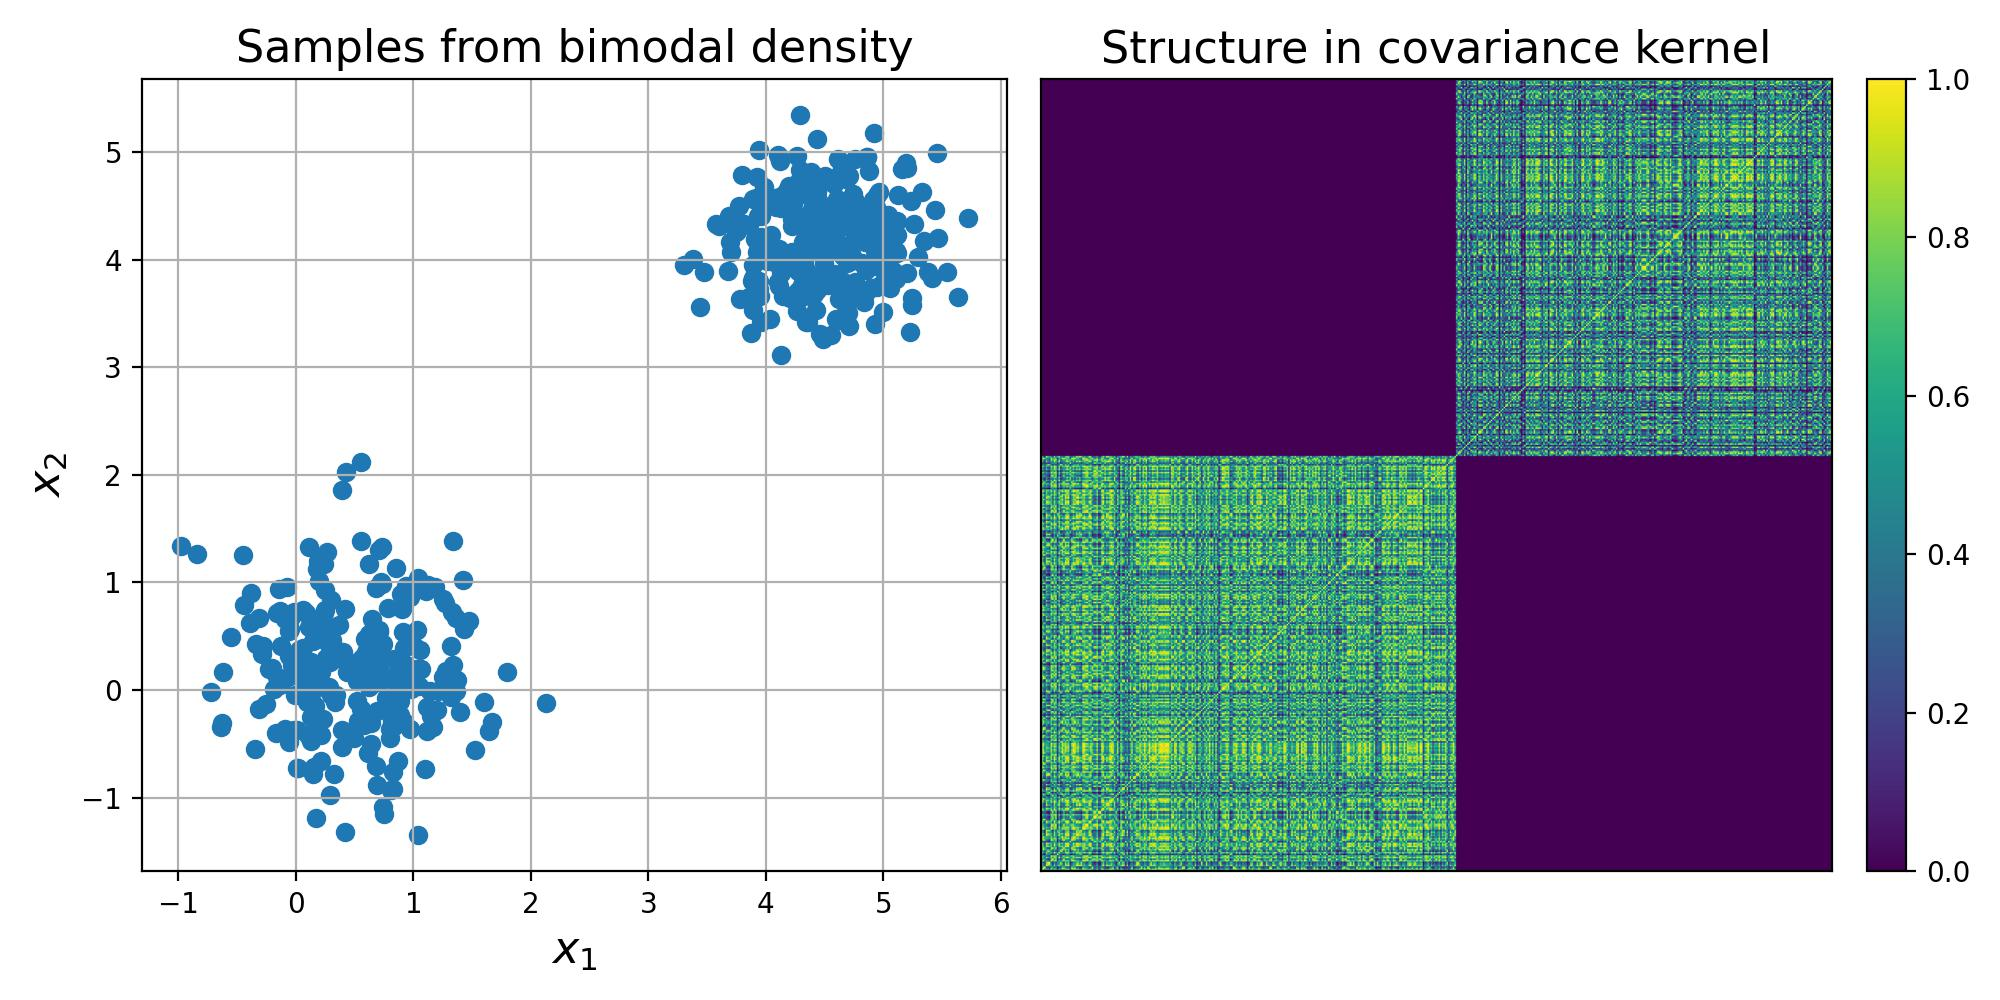
\includegraphics[width=0.75\linewidth]{figures/structure_cov_kernel.jpg}
    \caption{Covariance kernel with block diagonal structure corresponding to particles sampled from a bimodal target density}
    \label{fig:cov_structure}
\end{figure}

Estimation of sparse covariance structures \citep{fop_model-based_2018} is of great interest in the statistical literature and in studies of  graphical models. For instance, a message-passing version of SVGD \citep{wang_stein_2018} is tailored to continuous graphical models through localized kernel approximations. 

Our initial focus is on efficient evaluation of the score function through multi-fidelity setups that reduce the number of high-fidelity model-based likelihood evaluations, before considering a potential combination of the kernel and score approximation for future work.

\subsection{Gradient-based MCMC Methods}

SVGD differs from conventional gradient-based MCMC methods in its evolution of a co-ordinated particle ensemble instead of simulation of Markov chains with individual particles. In particular, the Euler-discretized Langevin dynamics simulates a Markov chain with the rule:

\begin{equation}
    x_{i+1} \leftarrow x_i + \frac{\epsilon}{2}\nabla \log p(x_i) + \epsilon \eta_i
\end{equation}

where $\eta_i \sim \CN(0, \epsilon)$ injects Gaussian noise at each step to prevent collapse to the MAP solution. 
For Bayesian inference, Stochastic Gradient Langevin Dynamics (SGLD) \citep{welling_bayesian_2011,brosse_promises_2018} permits use of large-scale datasets through unbiased gradient estimators based on small mini-batches of the data, potentially augmented with control-variates for variance reduction. 
While these approaches to Langevin dynamics are extremely relevant to discussions of variance reduction techniques for MCMC methods, the key ideas do not translate directly to the SVGD setting: instead of distributing workload amongst an ensemble of particles, these reduce the costs of likelihood evaluation conditioned on a particular realization of parameters $x$.


\subsection{Approximate Control Variates for Multi-fidelity Estimation}\label{ss: acv}

% \textcolor{red}{Stealing the text from acv with uq with some cuts}

Consider a mapping $Q=f_0(Z)$ that relates the random vector $Z \in \mathbb{R}^{n_{z}}$ and the random variable $Q \in \mathbb{R}$. The expected value of $Q$ is often approximated by a standard $N$-sample Monte Carlo (MC) estimator:
\begin{align}\label{eqn:mc}
    \mathbb{E}\left[Q_0\right] 
    \approx \hat{Q}_0 := \frac{1}{N} \sum^{N}_{j=1}f_0(z^{(j)}),
\end{align}

where $z^{(j)} \sim p(Z)$ are independent and identically distributed (i.i.d.) samples drawn from the probability distribution of $Z$. The MC estimator $\hat{Q}$ is unbiased, making its estimator error contributed entirely by its variance $N^{-1}\Var[Q]$. When using computationally intensive models, the number of samples $N$ that can be afforded may not be sufficiently high to limit this variance.

To reduce the estimator variance, multi-fidelity methods leverage an ensemble of low-fidelity models whose outputs are correlated with the high-fidelity model of interest but with diminished costs. 

Control variates (CVs) are a widely used classical method for variance reduction in Monte-Carlo methods. 
The general approach is to identify another function $f_1$, such that the traditional expected value estimator described in \autoref{eqn:mc} can be replaced by one constructed with $f_0 - f_1$, with smaller variance. The function $f_1$ is then referred to as a control variate. 
Typically, selection of $f_1$ (generalized to selection of $\{f_i\}, i=1, \cdots, M$) and identifying a rich set of candidate CVs is a non-trivial procedure barring the exceptions where CVs can be identified from domain knowledge. 
Linear transformations of the score function have been one of the popular choices given the high canonical correlations with the target that result in better variance reduction, and their straightforward incorporation into modern MCMC methods with gradient information and marginalization of hyperparameters \citep{papamarkou_zero_2014,oates_control_2017}. \cite{si_scalable_2021} extends CV identification to the high-dimensional settings by proposing a variational formulation based on Stein operators.
% \footnote{\textcolor{red}{Technically these are control functionals rather than control variates? \citep{oates_control_2017}}}.


In the context of multifidelity methods however, we typically already have access to a hierarchy of models, where each available low-fidelity model can be leveraged as a control variate, but their respective expectations must be computed from samples too. The approximate control variate (ACV) technique \cite{Gorodetsky2020, bomarito_optimization_2022} provides a rigorous formulation for deriving reduced-variance estimators in this setting.
This method introduces $M$ auxiliary random variables $Q_{m}$ for $m=1,\ldots,M$ that are outputs of the corresponding (e.g., low-fidelity) models $Q_{m} =f_{m}(Z)$, then combines the corresponding MC estimates of each low-fidelity model, $\hat{Q}_{m}$, into a single estimator. The ACV estimator, which we denote $\tilde{Q}$, can be written as:
\begin{align}
        \Tilde{Q}(z,\alpha,\CA) &:= 
        \hat{Q}_{0}(z_{0})+\sum^{M}_{m=1}\alpha_{m}\left( \hat{Q}_{m}(z^{\ast}_{m})-\hat{\mu}_{m}(z_{m}) \right) \nonumber\\ 
        &= \hat{Q}_{0}(z_{0})+\sum^{M}_{m=1}\alpha_{m}\left( \hat{Q}_{m}(z^{\ast}_{m})-\hat{Q}_{m}(z_{m}) \right),     \label{eqn:ACV-Formula}
\end{align}
where $\hat{\mu}_{m}$ is an MC estimate for the $m$th model mean, $\alpha = \left[ \alpha_{1}, \ldots, \alpha_M \right]$ is a vector of control variate weights, and the input samples $z$ are partitioned into subsets $z_{0}$, $z_{m}$, and  $z^{\ast}_{m}$ according to a sample partitioning strategy $\CA$. The control variate weights $\alpha$ and the sample partitioning strategy $\CA$ are hyperparameters of the estimator.
%that are chosen to optimally reduce the estimator variance. 

Since the ACV estimator is unbiased with respect to the high-fidelity model, its error is equal to the estimator variance. To express this variance mathematically, we introduce a vectorized notation for the ACV estimator:
\begin{align}\label{eqn:vectorized-acv}
    \Tilde{Q}(z;\alpha,\CA) = \hat{Q}_{0} + \alpha^{\top}\Delta,
\end{align}
where $\Delta:=\left[ \Delta_{1}(z_{1}^{\ast},z_{1}), \ldots,  \Delta_{M}(z_{M}^{\ast},z_{M})\right]$, $\Delta_{m}(z_{m}^{\ast},z_{m}):=\hat{Q}_{m}(z^{\ast}_{m})-\hat{Q}_{m}(z_{m})$, and the explicit dependence on the inputs $z_{m}$ and $z_{m}^{\ast}$ are omitted for simplicity of notation. The ACV estimator variance is then:
\begin{align}\label{eqn:acv-variance}
    \Var[\Tilde{Q}(z;\alpha,\CA)] = \Var[\hat{Q}_{0}] - \alpha^{\top}(\Cov[\Delta, \Delta])^{-1}\alpha + 2 \alpha^{\top} \Cov[\Delta, \hat{Q}_{0}].
\end{align}
The estimator variance is dependent on the covariances between each model output, the control variate weights, and the sample partitioning that influences how each $\Delta$ term covaries with each other and with $\hat{Q}_{0}$. If the exact covariance between each model output is known, then the optimal weights for a given ACV sample allocation $\CA$ can be computed by minimizing \eqref{eqn:acv-variance}. The optimal weights are:
\begin{align}\label{eqn:alpha-star-acv}
    \alpha^{\ast}(\CA)=-\Cov[\Delta, \Delta]^{-1}\Cov[\Delta, \hat{Q}_{0}],
\end{align}
and when these weights are set to their optimal values, the ACV estimator variance is~\cite{Gorodetsky2020}:
\begin{align}\label{eqn:acv-variance-opt}
    \Var[\Tilde{Q}^{\alpha^{\ast}}](\CA) = \Var[\hat{Q}_{0}] - \Cov[\Delta, \hat{Q}_{0}]^{\top} \Cov[\Delta, \Delta]^{-1}\Cov[\Delta, \hat{Q}_{0}].
\end{align}

The sample partitioning $\CA$ determines how much computational workload is distributed to each model. The well-known multi-fidelity Monte Carlo (MFMC) \cite{peherstorfer_optimal_2016} and multi-level Monte Carlo (MLMC) \cite{giles_multilevel_2015} methods can be shown to be special cases of ACV that differ in the family of possible $\CA$ choices. Solving for the optimal sample partitioning strategy $\CA^{\ast}$ is more intensive than solving for the optimal weights $\alpha^{\ast}$ but many tools \cite{bomarito_multi_2020, jakeman_pyapprox_2023} are available to approximately solve the optimization problem:
\begin{align}
    \min_{\mathcal{A}\in\mathbb{A}} &\quad \Var[\tilde{Q}(Z;\alpha^{\ast},\mathcal{A})] \label{eqn:mxmcpy}\\
    \text{subject to} &\quad \mathcal{W}(w,\mathcal{A})\leq w_{\text{budget}},\label{eqn:mxmcpy_constraint}
\end{align}
where $\mathbb{A}$ is a wide set of predefined allowable set of sample allocations, $w_{\text{budget}}$ is the total budget constraint, and $\mathcal{W}(w,\mathcal{A})$ computes the total cost of the estimator under model costs $w := [w_0, \ldots, w_M]$ and sample allocation $\CA$.

Importantly, the solutions to \eqref{eqn:mxmcpy} and \eqref{eqn:alpha-star-acv} are only computable with knowledge of the model output covariance matrix, $\Sigma = \Cov\left[ f_0(Z),\ldots,f_M(Z)
\right]$, as well as the model costs vector $w$. 
While the relationship between $\alpha$ and the estimator variance is clear from \eqref{eqn:acv-variance}, the relationship between $\Sigma$ and the estimator variance is dependent on $\CA$ via the terms in \eqref{eqn:acv-variance}:
\begin{align}
    \Cov[\Delta, \Delta] &= G(\CA) \odot \Sigma, \label{eqn:cov-delta-delta} \\
    \Cov[\Delta, \hat{Q}_{0}] &= \text{diag}(G(\CA)) \odot \text{col}_0( \Sigma ), \label{eqn:cov-delta-Q}
\end{align}
where $G \in \RR^{M\times M}$ is matrix that depends on $\CA$ and the exact sample allocation strategy in use (see \cite{bomarito_multi_2020}), $\odot$ signifies the Hadamard (elementwise) product, and $\text{col}_{0}( \Sigma )$ is the first column of $\Sigma$, i.e., the covariances between the high-fidelity model and all the low-fidelity models.
% While the model costs may often be known ahead of time, it is unlikely that the covariance matrix $\Sigma$ would be known \textit{a priori}. Traditionally, a set of $N_{\text{pilot}}$ independent pilot samples are used to compute an approximate covariance matrix $\hat{\Sigma}$ via the unbiased sample covariance formula:
% \begin{align}\label{eqn:cov}
%     \hat{\Sigma} = \frac{1}{N_{\text{pilot}}-1}\sum_{j=1}^{N_{\text{pilot}}}\left( f^{(j)} - \overline{f} \right) \left( f^{(j)} - \overline{f} \right)^{\top},
% \end{align}
% \sloppy where 
% %$N_{\text{pilot}}$ denotes the number of pilot samples, 
% $f^{(j)}=[ f_{0}(z^{(j)}),\ldots,f_{M}(z^{(j)}) ]^{\top}$, $\overline{f}=[ \overline{f}_{0},\ldots,\overline{f}_{M} ]^{\top}$, and $\overline{f}_{m}=\frac{1}{N_{\text{pilot}}}\sum_{j=1}^{N_{\text{pilot}}}f_{m}(z^{(j)})$. Too few pilot evaluations can lead to inaccurate covariance estimates and thus suboptimal ACV hyperparameters and high ACV errors. On the other hand, too many pilot evaluations can carry too much cost and leave too little computational budget left for the actual ACV estimator evaluation. While this trade-off has been investigated empirically in existing ACV literature~\cite{Peherstorfer2016, Gorodetsky2020}, a rigorous method is needed to help balance covariance uncertainty and pilot sampling budget. 



Alternative sampling-based estimators beyond the ACV formulation above, such as the multilevel best linear unbiased (MLBLUE) estimator from \cite{schaden_multilevel_2020} 
can produce impressive variance reduction like ACV. 
In fact, the generalized linear grouped ACV estimator (GACV) \cite{gorodetsky_grouped_2024} generalizes these methods. Though exact parametrizations may differ across estimators, they share common features of estimator weights and sample allocations.

% While MLBLUE and GACV are competitive with and can outperform ACV in some cases, we nonetheless use ACV in this work since potential performance improvements may be marginal relative to the issue of optimal pilot sampling. Importantly, the issue of covariance estimation still applies to these other estimators, and the pilot sampling termination algorithm presented in this paper can be applied to these other estimators by replacing the above variance formulae with their corresponding equations from \cite{gorodetsky_grouped_2024}.

% \subsection{Bayesian Optimal Experimental Design}



% \subsection{Flow Matching}

% Below, we briefly review the current practice in conditional flow matching algorithms and motivate their use in learning maps between samples from multiple-fidelity model likelihoods.

% Generative modeling tasks consider the problem of approximating and sampling from a probability distribution. For instance, continuous normalizing flows (CNFs) proposed in \cite{grathwohl_ffjord_2018} express an invertible mapping between a fixed and tractable source distribution and the data distribution using Neural Ordinary Differential Equations (NODEs). CNFs can be trained and scaled to larger datasets better through a regression of the ODE drift, a so-called Flow Matching (FM) objective. The advances proposed in \cite{tong_improving_2024} generalize the flow matching framework proposed by \cite{lipman_flow_2023} to use transport maps between arbitrary distributions and approximate the dynamic Optimal Transport problem during sampling of conditional paths to improve the efficiency of training and inference. 

% A smooth time-varying vector field $u: [0, 1] \times \RR^d \to \RR^d$ is defined by the following ordinary differential equation (ODE):
% \begin{equation}
%     dx = u(t, x)dt
% \end{equation}

% Given density $p_0$ over $\RR^d$, if $\phi_t(x)$ is the solution for the above ODE (i.e. it denotes the position of point $x$ transported along $u$ from time $0$ up to time $t$), this integration map introduces a pushforward density $p_t$ ($p_t$ is the density of points $x \sim p_0$ transported along $u$ from time 0 to time $t$) that is characterized by the continuity equation:

% \begin{equation}
%     \frac{\partial p}{\partial t} = -\grad.\left(p_t u_t\right)
% \end{equation}

% We can characterize the marginal probability path $p_t$ as a mixture of conditional probability paths:

% \begin{equation}
%     p_t(x) = \int p_t(x | z) q(z) dz
% \end{equation}

% If a path $p_t(x|z)$ is generated from $u_t(x | z)$ from initial conditions $p_0(x | z)$, then the vector field $u_t(x)$ given by:

% \begin{equation}
%     u_t(x) = \EE_{q(z)}\left[\frac{u_t(x|z)p_t(x|z)}{p_t(x)}\right]\label{eq: marg_cond_velocity_field}
% \end{equation}

% generates probability path $p_t(x)$ from initial conditions $p_0(x)$.

% The key ideas behind flow matching rely on this connection between marginal vector fields and marginal probability paths to decompose the intractable marginal vector field into conditional vector fields.

% The original flow matching objective considered in \cite{lipman_flow_2023} is intractable for general source density $q_0$ mapping to target $q_1$:

% \begin{equation}
%     \CL_{\text{FM}}(\theta)= \EE_{t \sim \mathcal{U}(0, 1), x \sim p_t(x)} ||v_\theta(t, x) - u_t(x)||^2
% \end{equation}

% In the special case where the marginal densities $p_t(x) = \CN(x | \mu_t, \sigma_t^2)$ are Gaussian, a possible simple (but non-unique) ODE satisfies:

% \begin{equation}
%     \phi_t(x_0) = \mu_t + \sigma_t \left(\frac{x_0 - \mu_0}{\sigma_0}\right) \label{eq: gaussian_ode_sol}
% \end{equation}

% and the unique vector field whose integration map satisfies \eqref{eq: gaussian_ode_sol} has the form:

% \begin{equation}
%     u_t(x) = \frac{\sigma_t'}{\sigma_t} (x - \mu_t) + \mu_t' \label{eq: vector_field_gauss_dens}
% \end{equation}

% where $\sigma_t'$ and $\mu_t'$ denote the time derivatives of $\sigma_t$ and $\mu_t$ respectively, and the vector field $u$ with initial conditions $\CN(\mu_0, \sigma_0^2)$ generates the Gaussian probability path $p_t(x) = \CN(x | \mu_t, \sigma_t^2)$.

% The flow matching loss under assumptions of existence and exchange of different integrals, and boundedness of the solution fields can be switched out for an easier-to-regress conditional flow matching loss with the loss gradient only changing by a constant factor that is independent of $\theta$:

% \begin{equation}
%     \CL_{\text{CFM}}(\theta) = \EE_{t, q(z), p_t(x|z)}||v_\theta(t, x) - u_t(x|z)||^2 \label{eq: cfm_loss}
% \end{equation}

% For all practical purposes, we can solve the much more useful CFM objective, under the condition that we can:

% \begin{enumerate}
%     \item Sample from $q(z)$

%     \item Sample from $p_t(x|z)$

%     \item Calculate $u_t(x|z)$
% \end{enumerate}

% \begin{equation}
%     \nabla_{\theta}\CL_{\text{FM}}(\theta) =\nabla_{\theta}\CL_{\text{CFM}}(\theta) \label{eq: cfm_fm_grad}
% \end{equation}

% A short proof of this is provided below from \cite{tong_improving_2024}:

% \begin{align*}
%     \grad_{\theta}\EE_{p_t(x)}||v_\theta(t, x) - u_t(x)||^2 &= \grad_\theta \EE_{p_t(x)}(||v_\theta(t, x)||^2 - 2\langle v_\theta(t, x) u_t(x)\rangle) \quad \textcolor{red}{\text{($u_t(x)
%     $ does not depend on $\theta$})}
% \end{align*}


% \begin{align*}
%     \grad_{\theta}\EE_{q(z),p_t(x|z)}||v_\theta(t, x) - u_t(x, z)||^2 &= \EE_{q(z), p_t(x|z)}\grad_{\theta}(||v_\theta(t, x)||^2 - 2 \langle v_\theta(t, x) , u_t(x|z)\rangle)
% \end{align*}

% The first term in each loss function can be reparametrized as:
% \begin{equation*}
%     \EE_{p_t(x)}||v_\theta(t, x)||^2 = \iint ||v_\theta(t, x)||^2 p_t(x|z)q(z)dz dx = \EE_{q(z), p_t(x|z)}||v_\theta(t, x)||^2
% \end{equation*}

% while we substitute \eqref{eq: marg_cond_velocity_field} in the inner product expression for FM to recover the CFM inner product and thus equalize the loss gradients:

% \begin{align*}
%     \EE_{p_t(x)}\langle v_\theta(t, x), u_t(x)\rangle &= \int \biggl<v_\theta(t, x), \frac{\int u_t(x|z)p_t(x|z)q(z)dz}{p_t(x)}\biggr>p_t(x)dx \\
%     &=\iint \langle v_\theta(t, x), u_t(x|z)\rangle p_t(x|z)q(z)dzdx \quad \textcolor{red}{\text{(inner product distributed over integral argument)}}\\
%     &=\EE_{q(z), p_t(x|z)}\langle v_\theta(t, x) u_t(x | z) \rangle
% \end{align*}

% \medskip
% \emph{I-CFM (via Independent Coupling):}
% For source point $x_0$ and target point $x_1$:

% \begin{enumerate}
%     \item $q(z) = q(x_0)q(x_1)$

%     \item $p_t(x|z) = \CN(x | tx_1 + (1 - t)  x_0, \sigma^2)$

%     \item Using \eqref{eq: vector_field_gauss_dens} for the conditional vector field with $\mu_t = tx_1 + (1 - t)x_0 $ and $\sigma_t = \sigma$, $u_t(x|z) = x_1 - x_0$
% \end{enumerate}

% \medskip
% \emph{OT-CFM (sampling via OT Map):}

% The key difference from I-CFM is that instead of $x_0, x_1$ being sampled independently from their marginal distributions, they are sampled jointly according to the optimal transport map $\pi$:

% $$q(z) = \pi(x_0, x_1)$$

% In cases where a static OT plan is computationally infeasible to determine exactly, a minibatch OT approximation \citep{fatras_learning_2020} shows improvements over random sampling plans in terms of model performance and training times. 
% Related work such as that of \cite{finlay_how_2020} use a regularized CNF with dynamic OT objectives though these are difficult to train and scale.


% \emph{SB-CFM (entropy-regularized OT map):}
% Recent efforts such as \citep{de_bortoli_diffusion_2021,heng_diffusion_2024} have also focused on efficient inference in diffusion models and general Bayesian computation by reformulating them as a Schrödinger bridge (SB) problem where the forward process need not be run for large number of steps to ensure $p_N = p_{\text{prior}}$. 
% The static SB problem can be seen as an entropy-regularized quadratic cost OT problem that is an attractive choice for high-dimensional OT between arbitrary data distributions. 
% These can be applied to an entropic variant of OT-CFM, SB-CFM, to match probability flow of a Schrödinger bridge with a Brownian motion refererence process.

% The SB problem seeks a process $\pi$ that is closest to the initial time marginal $p_{\text{ref}}$ while having initial and terminal marginal distributions specified by $q(x_0)$ and $q(x_1)$ respectively i.e.:
% \begin{equation*}
% \pi^{\ast} = \argmin_{\pi(x_0) = q(x_0), \pi(x_1)=q(x_1)} \DKL(\pi, p_{\text{ref}})
% \end{equation*}

% Then the above solution can be recovered through the marginal vector field $u_t(x)$ defined via:

% \begin{enumerate}
% \item $q(z) = \pi_{2\sigma^2}(x_0, x_1)$ where $\pi_{2\sigma^2}(x_0, x_1)$ solves the entropy-regularized optimal transport problem with cost $||x_0 - x_1||$ and regularization $\lambda = 2\sigma^2$

% \item $p_t(x|z) = \CN(x | tx_1 + (1 - t)x_0, t(1-t)\sigma^2$ \textcolor{red}{(Brownian bridge between $x_0$ and $x_1$)}

% \item $u_t(x|z) = \frac{1 - 2t}{2t(1-t)}\left(x - (tx_1 + (1 - t) x_0) \right) + (x_1 - x_0)$
% \end{enumerate}

% The ability to establish correlations through reasonably sized pilot datasets may be enhanced through the use of flow matching. 
% In cases where the high-fidelity model can only be evaluated a limited number of times, the flow matching surrogate can enable a fast mapping from the particles propagated under a lower-fidelity model likelihood to those under the highest fidelity likelihood. 
% Moreover, it can be parametrized to use particles based on multiple lower-fidelity models for even greater savings.

\section{Methodology}

Given access to a model ensemble $f_i(x)$, $i=1, \cdots, M$ where the subscript indexes models from the highest to the lowest fidelity, and $x \in \RR^{n_x}$ is a random vector, the data-generating process and the log-likelihood functions corresponding to these outputs can be expressed as:


% Let $y_0$ and $y_1$ be observations 


% \begin{equation}
%     y_i^{(j)} = f_i(\theta)^{(j)} + \varepsilon_i
%     \label{eq: dgp_fid}
% \end{equation}

% where \varepsilon is homoskedastic noise associated with  


\begin{align}
 y_i = f_i(x) + \epsilon_i, \qquad L_i = \log p(\mathbf{y}_i | x) = \prod_{k=1}^N \log p(y_k | x)
 \label{eq: lik_fid_dgp}
\end{align}

where $\mathbf{y}_i = [y_1, \cdots, y_k, \cdots, y_N]$ are i.i.d. observations and $\epsilon_i$ is zero-mean additive noise.

Using the same prior density $p_o(x)$ in each of the inference setups for the individual models, the score function for the posterior PDF then simplifies to the following tractable expression that does not require evaluation of the normalizing constant:

\begin{align}
    \nabla_{x} \log p_i(x \mid D) = \nabla_x (L_i  + \log(p_o(x)),
    \label{eqn: bayes_rule_score}
\end{align}

\subsection{Baseline: Bifidelity SVGD}


% Then assuming an additive correction, a simple Stein update for the parameters $\theta_i$ would become:

Before we propose the multi-fidelity construction, it is is still instructive to demonstrate the basic idea of partitioning the likelihood evaluation costs through a bifidelity surrogate SVGD construction, where a subset of particles evaluated under the lower-fidelity target density are `corrected' through the corresponding high-fidelity density gradient update.

Let $n_0$ be the number of particles that are updated under both high and low-fidelity likelihood models. Let $n_1$ represent the number of particles updated only under the low-fidelity representation.

Then the new updates take the form:
\begin{align}
    x_i^{l + 1} &\leftarrow x_i^l + \epsilon_l\hat{\phi}^{\ast}_{\text{BF}}(x_i^l)
    \label{eq: bf_svgd_basic}
\end{align}

where:
\begin{align}
    \hat{\phi}^{\ast}_{\text{BF}}(x) &= \frac{1}{n_1}\left[\sum_{j=1}^{n_1} k(x_j^l, x) \nabla_{x_j^l}\log p_1(x_j^l) + \nabla_{x_j^l}k(x_j^l, x)\right]
    + \frac{1}{n_0}\left[\sum_{j=1}^{n_0} k(x_j^l, x) \nabla_{x_j^l}\log \left(\frac{p_0(x_j^l)}{p_1(x_j^l)}\right)\right]
    \label{eq:bf_gradient_expr}
\end{align}

The key features of the update are:

\begin{enumerate}
    \item The correction term does not contain a repulsive force term, and the repulsion term in the first half of the equation has to accomodate particles updated under a single as well as multiple fidelities.

    \item The magnitudes of the score difference are smeared over the domain through the correlations between the high-fidelity and the remainder of the low-fidelity particles. 

    \item The subset of particles used to define the correction term is \emph{randomized} from iteration to iteration. This is key to all particle positions eventually correcting to fit the target high-fidelity density.
\end{enumerate}

% While we do not draw directly from the theory of numerical methods and ODE integrators


% The additive correction is learnt subsets that are randomized from iteration to iteration. In this case, the repulsion term is driven by particle positions under the misspecified likelihood during the initial step and a mixture of particles driven by multiple fidelities in subsequent steps.

A quality measure is needed to determine when a sequence of samples is converging or not to the target density in SVGD. Stein's method provides a tool to define a discrepancy measure between densities $p$ and $q$ that can measure asymptotic bias in approximate MCMC samplers \cite{gorham_measuring_2017} and is also tailored to SVGD-based inference.\footnote{A key benefit is the ability to evaluate the discrepancy without explicit density estimation of $q$ for the propagated particles, unlike the more popular KL-divergence.} For smooth functions $f(x) \in \CF$, the Stein discrepancy measure\citep{liu_kernelized_2016} is defined as :

\begin{equation}
    \mathbb{S}(q, p) = \max_{f \in \CF}\left(\EE_q[\nabla_x \log p(x)f(x) + \nabla_x f(x)]\right)^2 \label{eq:ksd_regular}
\end{equation}

\cite{liu_kernelized_2016} define a computationally tractable version of this by assuming $\CF$ to be a ball in a reproducing kernel Hilbert space (RKHS) associated with a smooth positive definite kernel $k(x, x')$. Denoting $\nabla_x \log p(x)$ by $s_p$, the Kernelized Stein Discrepancy (KSD),

\begin{align}
    \mathbb{S}(q, p) &= \mathbb{E}_{x, x' \sim q}[u_p(x, x')] \nonumber \\ 
    &= \mathbb{E}_{x, x' \sim q}[s_p(x)^{\top} k(x, x')s_p(x') + s_p(x)^{\top} \nabla_{x'}k(x, x') + \nonumber\\ 
    & \nabla_x k(x, x')^{\top}s_p(x') + \operatorname{trace}(\nabla_{x, x'}k(x, x'))] \label{eq:ksd_kernel}
\end{align}

is the empirical evaluation of $\mathbb{S}(q, p)$, which can be estimated through the following $U$-statistic:

\begin{align}
    \hat{\mathbb{S}}_u(q, p) = \frac{1}{n(n-1)}\sum_{1 \leq i \neq j \leq n} u_p(x_i, x_j)
\end{align}

% \begin{align}
%     d_{\CH}(q, p) \triangleq
% \end{align}

% We assess the performance of each SVGD variant through the Kernelized Stein Discrepancy (KSD), which represents the maximum violation of Stein's identity when the expectation is computed under $q$ instead of $p$ and therefore avoids explicit integration under the target. 

Theory for the weak convergence of KSD is developed in \cite{gorham_measuring_2017}, and suggests that commonly used KSD formulations fail to detect non-convergence for violating sample sequences, even for simple Gaussian targets in small to modest dimensions ($d \geq 3$). 
In examples showcasing SVGD for higher dimensions, we use the Inverse Multiquadric (IMQ) Kernel i.e. $k(x, x') = (c^2 + ||x - x'||_2^2)^\beta$ instead of the RBF or Matern kernel in line with their recommendations, with $\beta=-1/2$ and $c=1$. A comparison of the IMQ and RBF kernel basis functions is shown in \autoref{fig:imq_vs_rbf}, with the RBF kernel defined as $k(x, x') = \exp(-||x - x'||_2^2 / h^2)$.

Our initial demonstrations do not specify an explicit prior and likelihood but instead evaluate the effectiveness of the proposed estimator on an ensemble of closed-form target density functions. We show an example of mapping from an initial set of particles to a Gaussian mixture high-fidelity target density, while leveraging a lower-fidelity density $p_1$ which corresponds to one of the modes.
\begin{align}
    p_1(\mathbf{x}) &= \CN\left(\mathbf{x}; \begin{bmatrix}-2.5 \\ -1.5\end{bmatrix}, \begin{bmatrix}1.5 & 0 \\ 0 & 0.5\end{bmatrix}\right)\\ \nonumber
    p_2(\mathbf{x}) &= \CN \left(\mathbf{x}; \begin{bmatrix}0.5 \\ 0.2\end{bmatrix}, \begin{bmatrix}2.0 & 0.3 \\ 0.3 & 0.5\end{bmatrix}\right)\\ 
    p_0(\mathbf{x}) &= \sum_{j=1}^2 \pi_j \CN(\mathbf{x}; \mu_j, \sigma_j) \quad, \pi_1 = \pi_2 = 0.5 \nonumber
    \label{eq:p0p1_toy_example}
\end{align}

\begin{figure}[H]
    \centering
    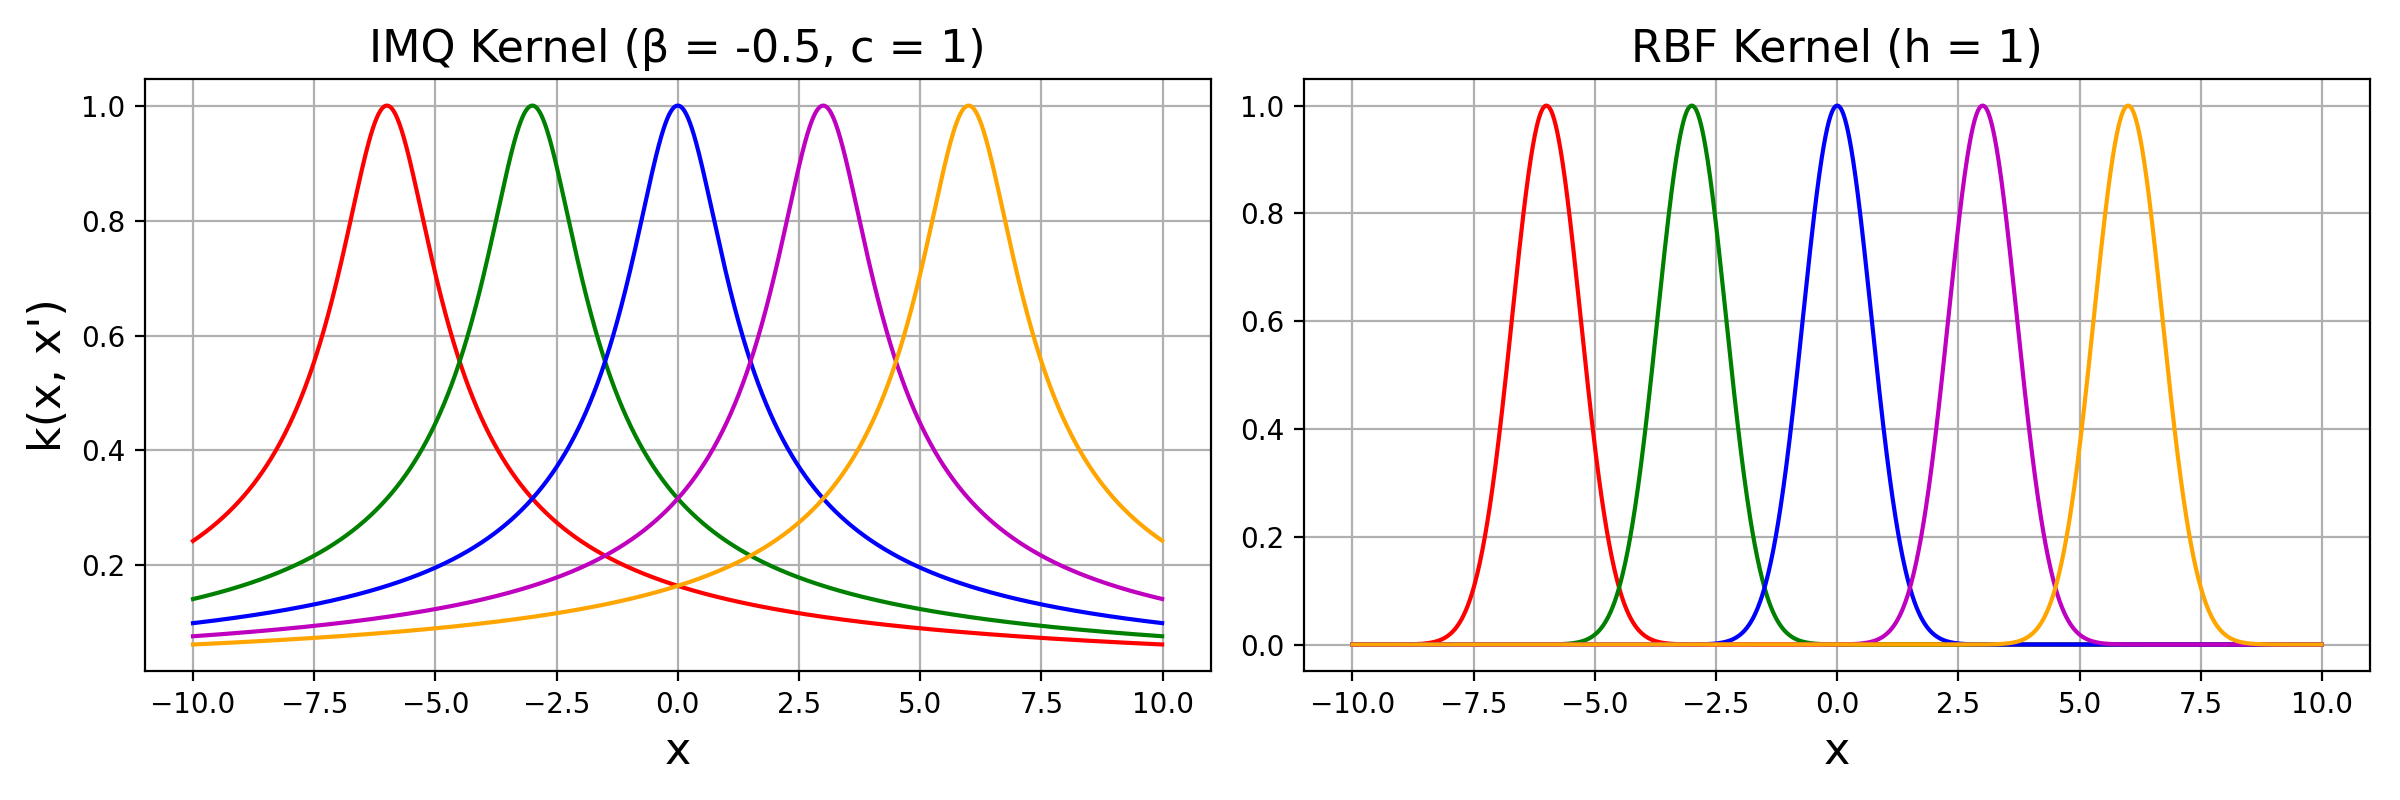
\includegraphics[width=0.85\linewidth]{figures/imq_vs_rbf_basis_functions.png}
    \caption{Examples of basis functions generated through IMQ and RBF kernels for $d=1$. The most significant difference is the smoothly decaying tails for RBF, which falls in the class of KSDs that may fail to detect non-convergence.}
    \label{fig:imq_vs_rbf}
\end{figure}


\begin{figure}[H]
    \centering
    % 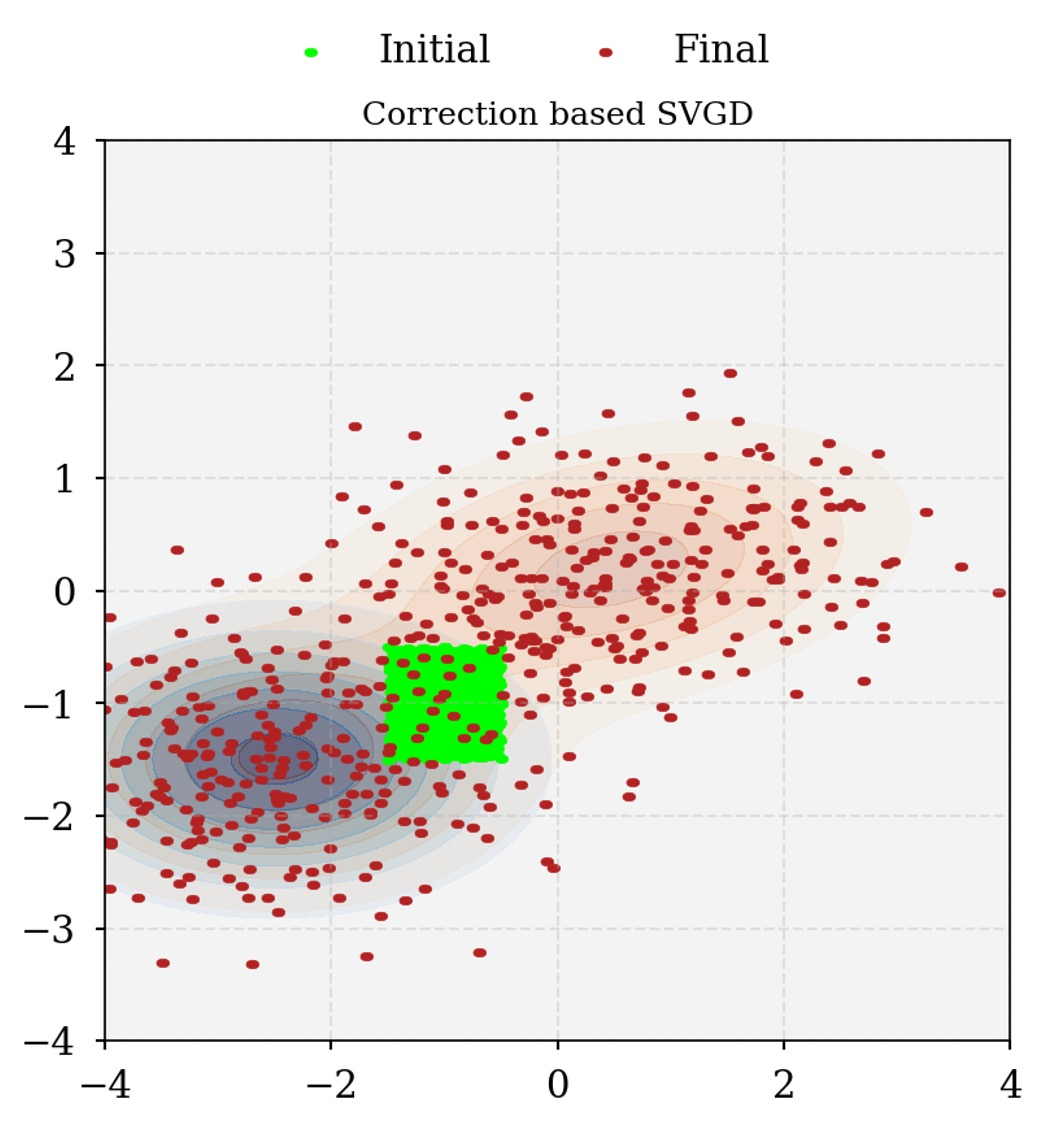
\includegraphics[width=0.75\linewidth]{figures/svgd_scalable_mixture_hf.jpg}
    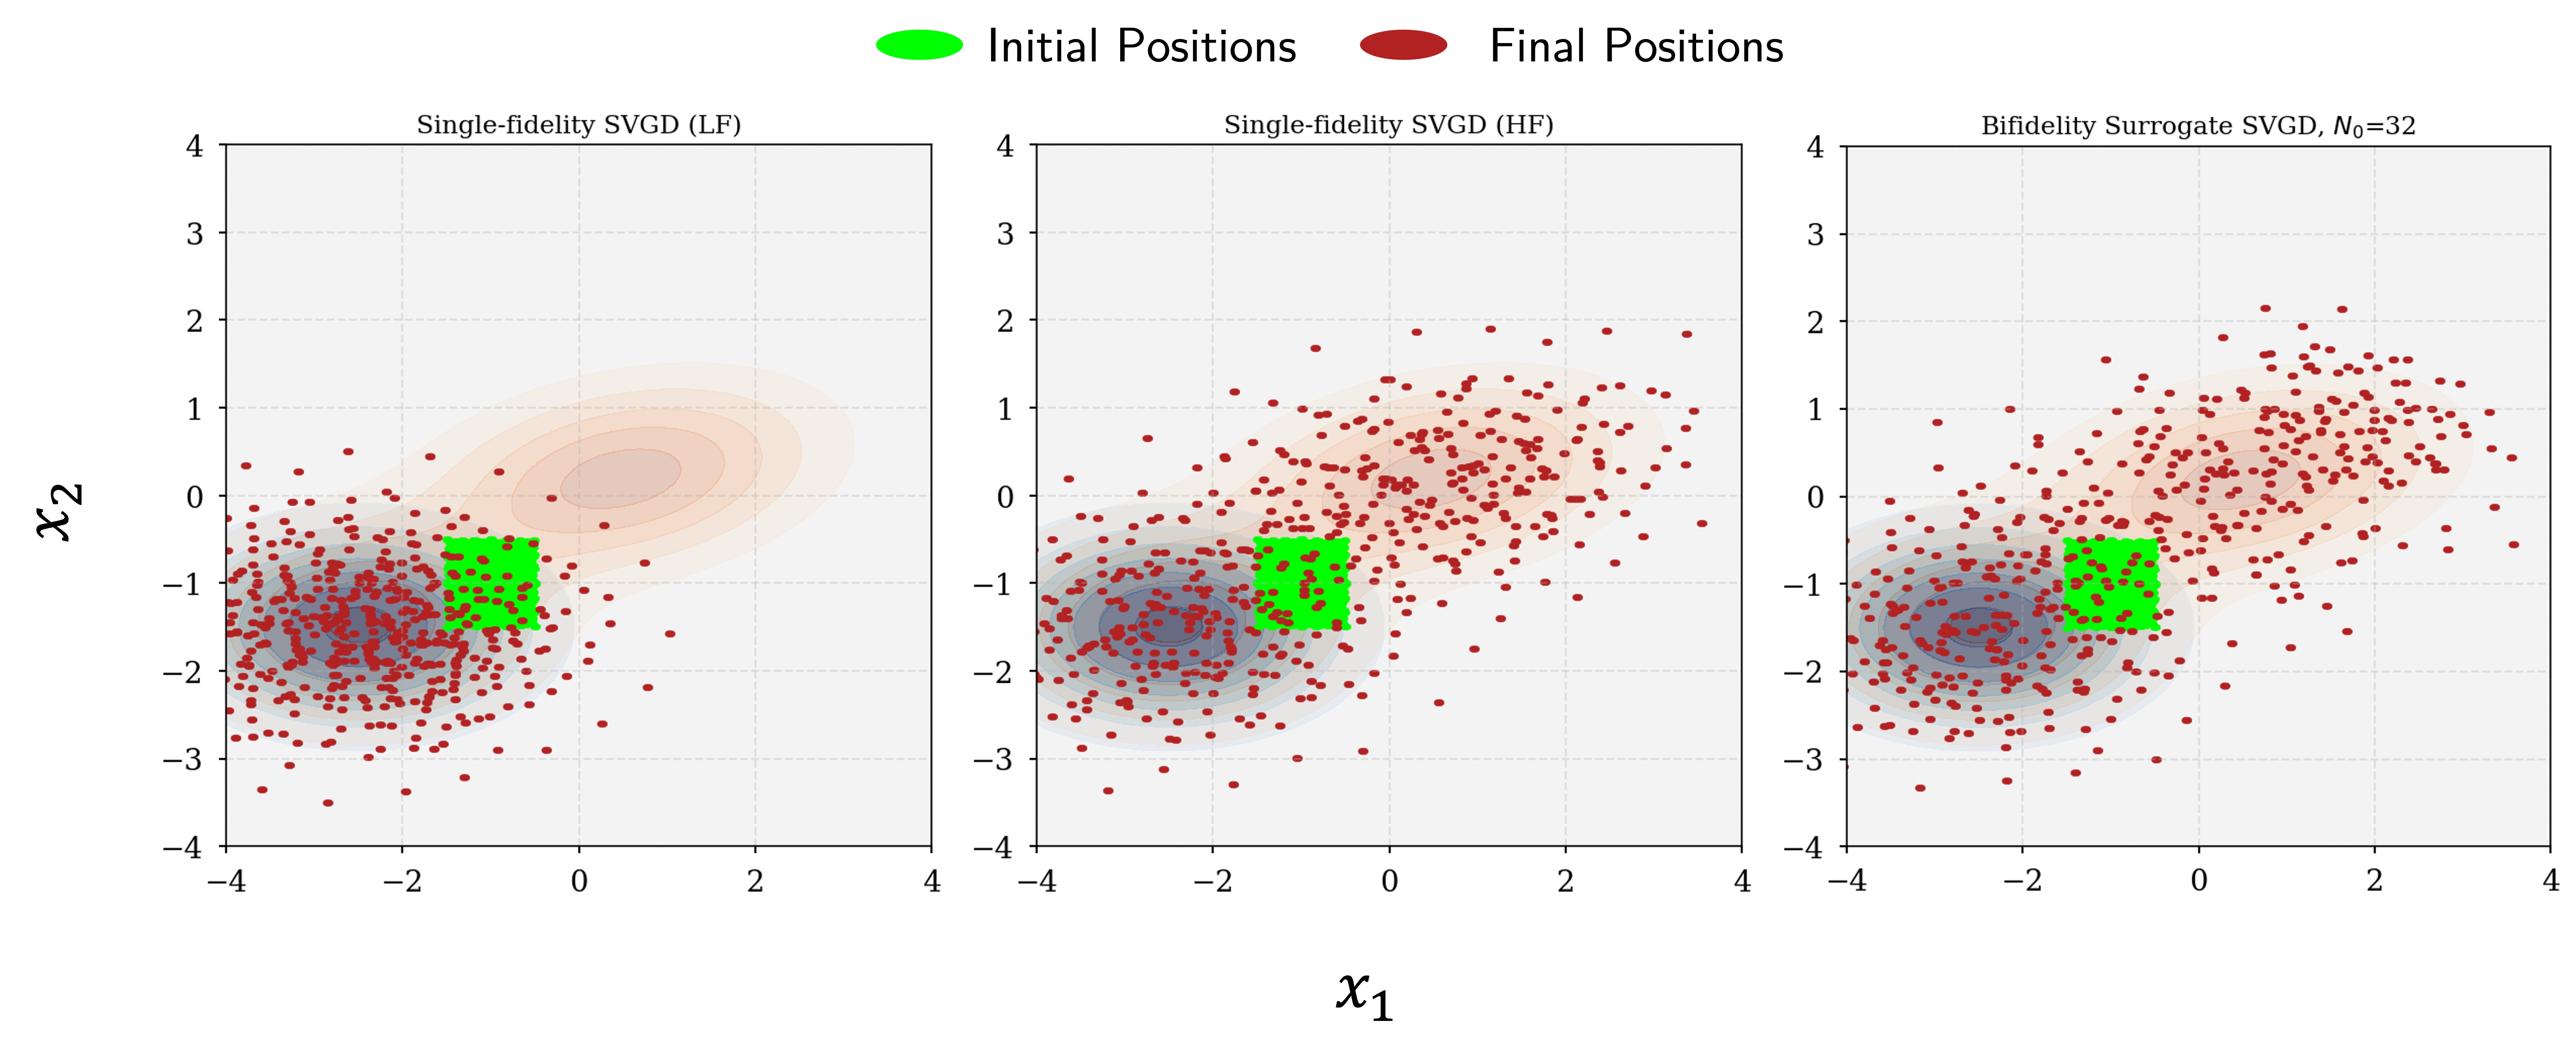
\includegraphics[width=\textwidth]{figures/bifidelity_svgd_comparisons_gaussian_mixture_rbf.jpg}
    \caption{Particles mapping to the high-fidelity target posterior based on the surrogate bifidelity gradient estimator for SVGD (right) and the single fidelity estimators under individual LF and HF targets (left and middle). The contours of the high-fidelity distribution, a Gaussian mixture, are marked in orange, while those of the unimodal lower-fidelity target are marked in blue. The particle positions at the initial timestep, drawn through quasi-MC uniform sampling, are marked in green, and those in brown represent the positions at the final timestep. 32 particles are used to correct the low-fidelity estimate at each step for the surrogate estimator.}
    \label{fig:svgd_sf_vs_bf_surrogate_rbf}
\end{figure}

Next, KSD is reported for target ensembles with total number of particles set to \textnormal{\{16, 32, 64, 128, 256, 512\}}
to measure the gap between the density induced by SVGD particles at the final update step and samples from the true posterior. We compare KSD trends for vanilla SVGD and the bifidelity-surrogate SVGD (BFS-SVGD), the latter with a varying number of particles used for the correction term.





% To better interpret the efficacy of the bifidelity update, we first visualize the evolution of the contributors to the velocity field i.e. SVGD gradient at different time steps.





% \textbf{Finite particle convergence for SVGD}

% \cite{shi_finite-particle_2023} establish the first finite particle convergence rates for SVGD. 






% \begin{equation}
%     \theta_i \leftarrow \theta_i + \epsilon \phi^{\ast}(\theta)
% \end{equation}

% where 

% \begin{equation}
%     \phi^{\ast}(\theta) = \frac{1}{M}\sum_{j=1}^{M}[k(\theta_j, \theta) \grad_{\theta_j}[(L_{1}(\theta_j) + L_{\Delta}(\theta_j) + \log p(\theta)] + \grad_{\theta_j} k(\theta_j, \theta)]
% \end{equation}

% While this framework does on the surface, construct an update equation based on multiple models, it comes with its fair share of drawbacks: for one, it requires us to propose an adequate estimator for $L_{\Delta}$, followed by a design for pilot samples to correlate the two models and a formal accounting of the bias introduced by this correction. 
% A viable strategy is to allocate model fidelities to individual particles, and construct an unbiased estimator of the gradient flow to target cost savings via limited and strategic querying of high-fidelity model / likelihood updates. 
% While not quite used for Bayesian inference, similar ideas have found traction in the field of rare event estimation \cite{dhulipala_bayesian_2022}, where the objective is to use the uncertainty from low-fidelity model outputs as an indicator of proximity of particles to the failure boundary. Following this, the limit state function can be computed through the higher-fidelity model and sample the boundary efficiently.

\subsection{Generalized Multifidelity-SVGD (MFS-SVGD)}

The most general form of a multi-fidelity update for SVGD would partition the incremental transform in the style of ACVs so that particles are apportioned to target densities of different fidelities for computing the incremental transform at every iteration. 
The key differences compared to the surrogate SVGD estimator we discussed in the previous section would stem from both the unbiasedness of the ACV estimator and the ability to accomodate arbitrary model ensembles with error-optimal particle allocations.

Following the notation introduced in \autoref{ss: acv}, we can propose different versions of a multi-fidelity SVGD framework depending on the computation of the different forces making up the usual SVGD gradient.

For a particle ensemble $\mathbf{x}^{(l)}$ at iteration $l$, , let $z_i^l=$\mathbf{x}^{(l)} \setminus x_i^l$. \textcolor{red}{Not strictly correct notation, but makes it easier to digest the following equations}

\begin{enumerate}
\item Collectively decomposing the kernel-weighted scores and the repulsive force terms:
\begin{align}
        \tilde{\phi}(x_i^l, z_i^l, \alpha, \CA) = \tilde{\phi_0}(x_i^l, z_0) + \sum_{m=1}^M \alpha_m \left(\hat{\phi}_m(x_i^l, z_m^{\ast}) - \hat{\mu}_m(x_i^l, z_m)\right)
\end{align}

followed by:
\begin{align}
    x_i^{l + 1} \leftarrow x_i^l + \epsilon_l\tilde{\phi}(x_i^l, z_i^l, \alpha, \CA)
    \label{eq: mf_svgd_proposal_1}
\end{align}
where the subscript in $\phi_{(\cdot)}$ denotes the model used in the gradient estimate with the usual decomposition for $\phi$.

\item Computing the repulsive force over all particles through usual single-fidelity MC without including it in the full multi-fidelity gradient estimator:
\begin{align}
        \tilde{\psi}(x_i^l, z_i^l, \alpha, \CA) = \tilde{\psi_0}(x_i^l, z_0) + \sum_{m=1}^M \alpha_m \left(\hat{\psi}_m(x_i^l, z_m^{\ast}) - \hat{\gamma}_m(x_i^l, z_m)\right)
\end{align}
followed by:
\begin{align}
    x_i^{l + 1} \leftarrow x_i^l + \epsilon_l\tilde{\psi}(x_i^l, z_i^l, \alpha, \CA) + \epsilon_l\left[\frac{1}{n}\sum_{j=1}^{n} \nabla_{z_j^l} k(z_j^l, x)\right]
    \label{eq: mf_svgd_proposal_2}
\end{align}
where $\tilde{\psi}_{(\cdot)}$ is shorthand for $\left[\frac{1}{n_{(\cdot)}} \sum_{j=1}^{n_{(\cdot)}}k(z_j^l, \cdot) \nabla_{z_j^l} \log p_{(\cdot)} (z_j^l)\right]$, the so-called `confining term' \citep{ye_stein_2020} and $n_i$ denotes the fraction of particles out of $n$ particles used in the score computation for model $i$.
\end{enumerate}

Other choices that we do not focus on here may construct separate MF estimators for each term of the gradient, or build a nested estimator, where the partitioning is performed for the kernel computations, followed by an additional allocation step to models of different fidelities. 
We leave exploration of the implications resulting from these choices to future work and discuss the above choices in greater detail as a first step towards a useful multi-fidelity algorithm.



\subsubsection{Offline Pilot Sampling}

As the particles initialized with density $q_0$ are propagated towards the target $p_i$, the ACV estimates need to be recomputed for every intermediate density $q_i$, ideally with a smaller subset of particles that can establish a fairly accurate estimate of the pilot covariance matrix. 

A method for offline pilot sampling is presented below. It relies on generating particles sequences under some choice of $p_i$ and number of pilot particles $N_p$. Then, keeping this sequence fixed, we recover the particle-wise weighted score function values at every step for all model fidelities. Finally, we summarize the particle-wise correlations based on the score function values to establish a fixed stepwise sample allocation. 

We will use the simplest variation of ACV for our ACV-SVGD based framework that computes multi-fidelity estimates for a single output / scalar QoI. This implies that for a $d$-dimensional target posterior, the sample allocations for each update directions are computed separately based on optimal variance reduction in the respective components of the gradient / velocity field. While this is by far the most scalable approach, there is also potential to exploit the correlations between gradient components for even greater variance reduction \citep{dixon_covariance_2024}. 




% The simplest method considers non-adaptivity of learning rates and correlations established through pilot sampling.

% \begin{algorithm}[ht!]
% \caption{Non-adaptive Pilot Sampling-based MF-SVGD}\label{alg:pilot_sampling_termination}
% \begin{algorithmic}[1]
% \item Pilot sampling loop - either: take a small set of particles propagated across all fidelities, and get the correlations from these. OR: we choose a specific fidelity, and obtain all the intermediate gradients. Then the question is: keeping these positions fixed, what are the operator action correlations for the remaining fidelities? 
% % \textcolor{red}{check! do these perform the same computation?}

% \item given stagewise correlations, determine particle allocations, compute respective updates and form ACV estimator.
% \end{algorithmic}
% \end{algorithm}

\begin{algorithm}[H]
  \caption{Offline Pilot Sampling}\label{alg: pilot_sampling_non_adaptive}
  \begin{algorithmic}[1]   
  \State \textbf{Input:} Step size $\epsilon$, densities $p_i(x)$ for $i=0,\dots,M-1$, kernel $k(x,x')$, initial particles $\{x_j^{(0)}\}_{j=1}^{N_p}$, total budget $B$.
  \State \textbf{Output:} Covariance matrix and sample allocations for $L$ iterations
  \State Choose fidelity $i$ to compute deterministic particle sequences for $L$ iterations with step size $\epsilon$, obtain sequence $S_x  = \{\mathbf{x}^{(0)}, \cdots, \mathbf{x}^{(L - 1)}\}$, where $\mathbf{x}^{(l)} = \{x_i^{(l)}\}_{i=1}^{N_p} \sim q^{(l)}$
  \State Using $S_x$, store gradient contributions to each particle from neighbour particles for each target density in the model ensemble at every step: $\Psi^{(j)} = \begin{bmatrix}
      k(x_1, x_1)\nabla_{x_1} \log p_j(x_1) & \cdots & k(x_{n_p}, x_1) \nabla _{x_{n_p}}\log_{x_{n_p}}p_j(x_{n_p}) \\
      \vdots & \vdots & \vdots \\
      k(x_1, x_{n_p})\nabla_{x_1} \log p_j(x_1) & \cdots & k(x_{n_p}, x_{n_p}) \nabla _{x_{n_p}}\log_{x_{n_p}}p_j(x_{n_p})
  \end{bmatrix}$ and $\Psi = \{\Psi^{(j)}\}_{j=0}^{M-1}$
  \State Obtain sample covariances $C_i^{(l)}$ for each particle using stored $\Psi^j$, and compute sequence of the mean covariance matrix $\{\hat{C}^{(l)}\}_{l=1}^{L}$ to set as ACV hyperparameters.
  \State Obtain stepwise sample allocations and control variate weights: $\alpha^l, \CA^l \leftarrow \texttt{ACVEstimator}(B, \hat{C}^{(l)})$
\end{algorithmic}
\end{algorithm}

An alternate approaches involves constructing a biased estimate of $\hat{C}^{(l)}$ by using gradients computed for all particles directly i.e. $K\nabla_{\mathbf{x}}\log p_i$. An example of the same is shown for an ensemble of Gaussian target densities, with $N_p=32$, $\epsilon=0.1$ and a synthetic cost vector $w=[1, 0.75, 0.25]$, from which the total budget is set to $B=64 \cdot \sum_i w_i$. The target $p_1$ is used to compute $S_x$.

In \autoref{fig:svgd_gaussians_pilot_corrs}, we show the log-densities of each of the ensemble members and the stepwise correlation estimates from the approach of \autoref{alg: pilot_sampling_non_adaptive} as well as the alternate approximation, the former of which is more conservative in the correlation estimates.

Our next steps will include testing various approaches to pilot sampling, including an online covariance estimation step, where a subset of propagated $N$ particles can be evaluated instead of an independent offline pilot set. 
Finally, single-output and multiple output ACV estimators will be compared alongside the surrogate bifidelity estimator in various settings to establish the efficacy of the multi-fidelity framework. 

\begin{figure}[H]
    \centering
    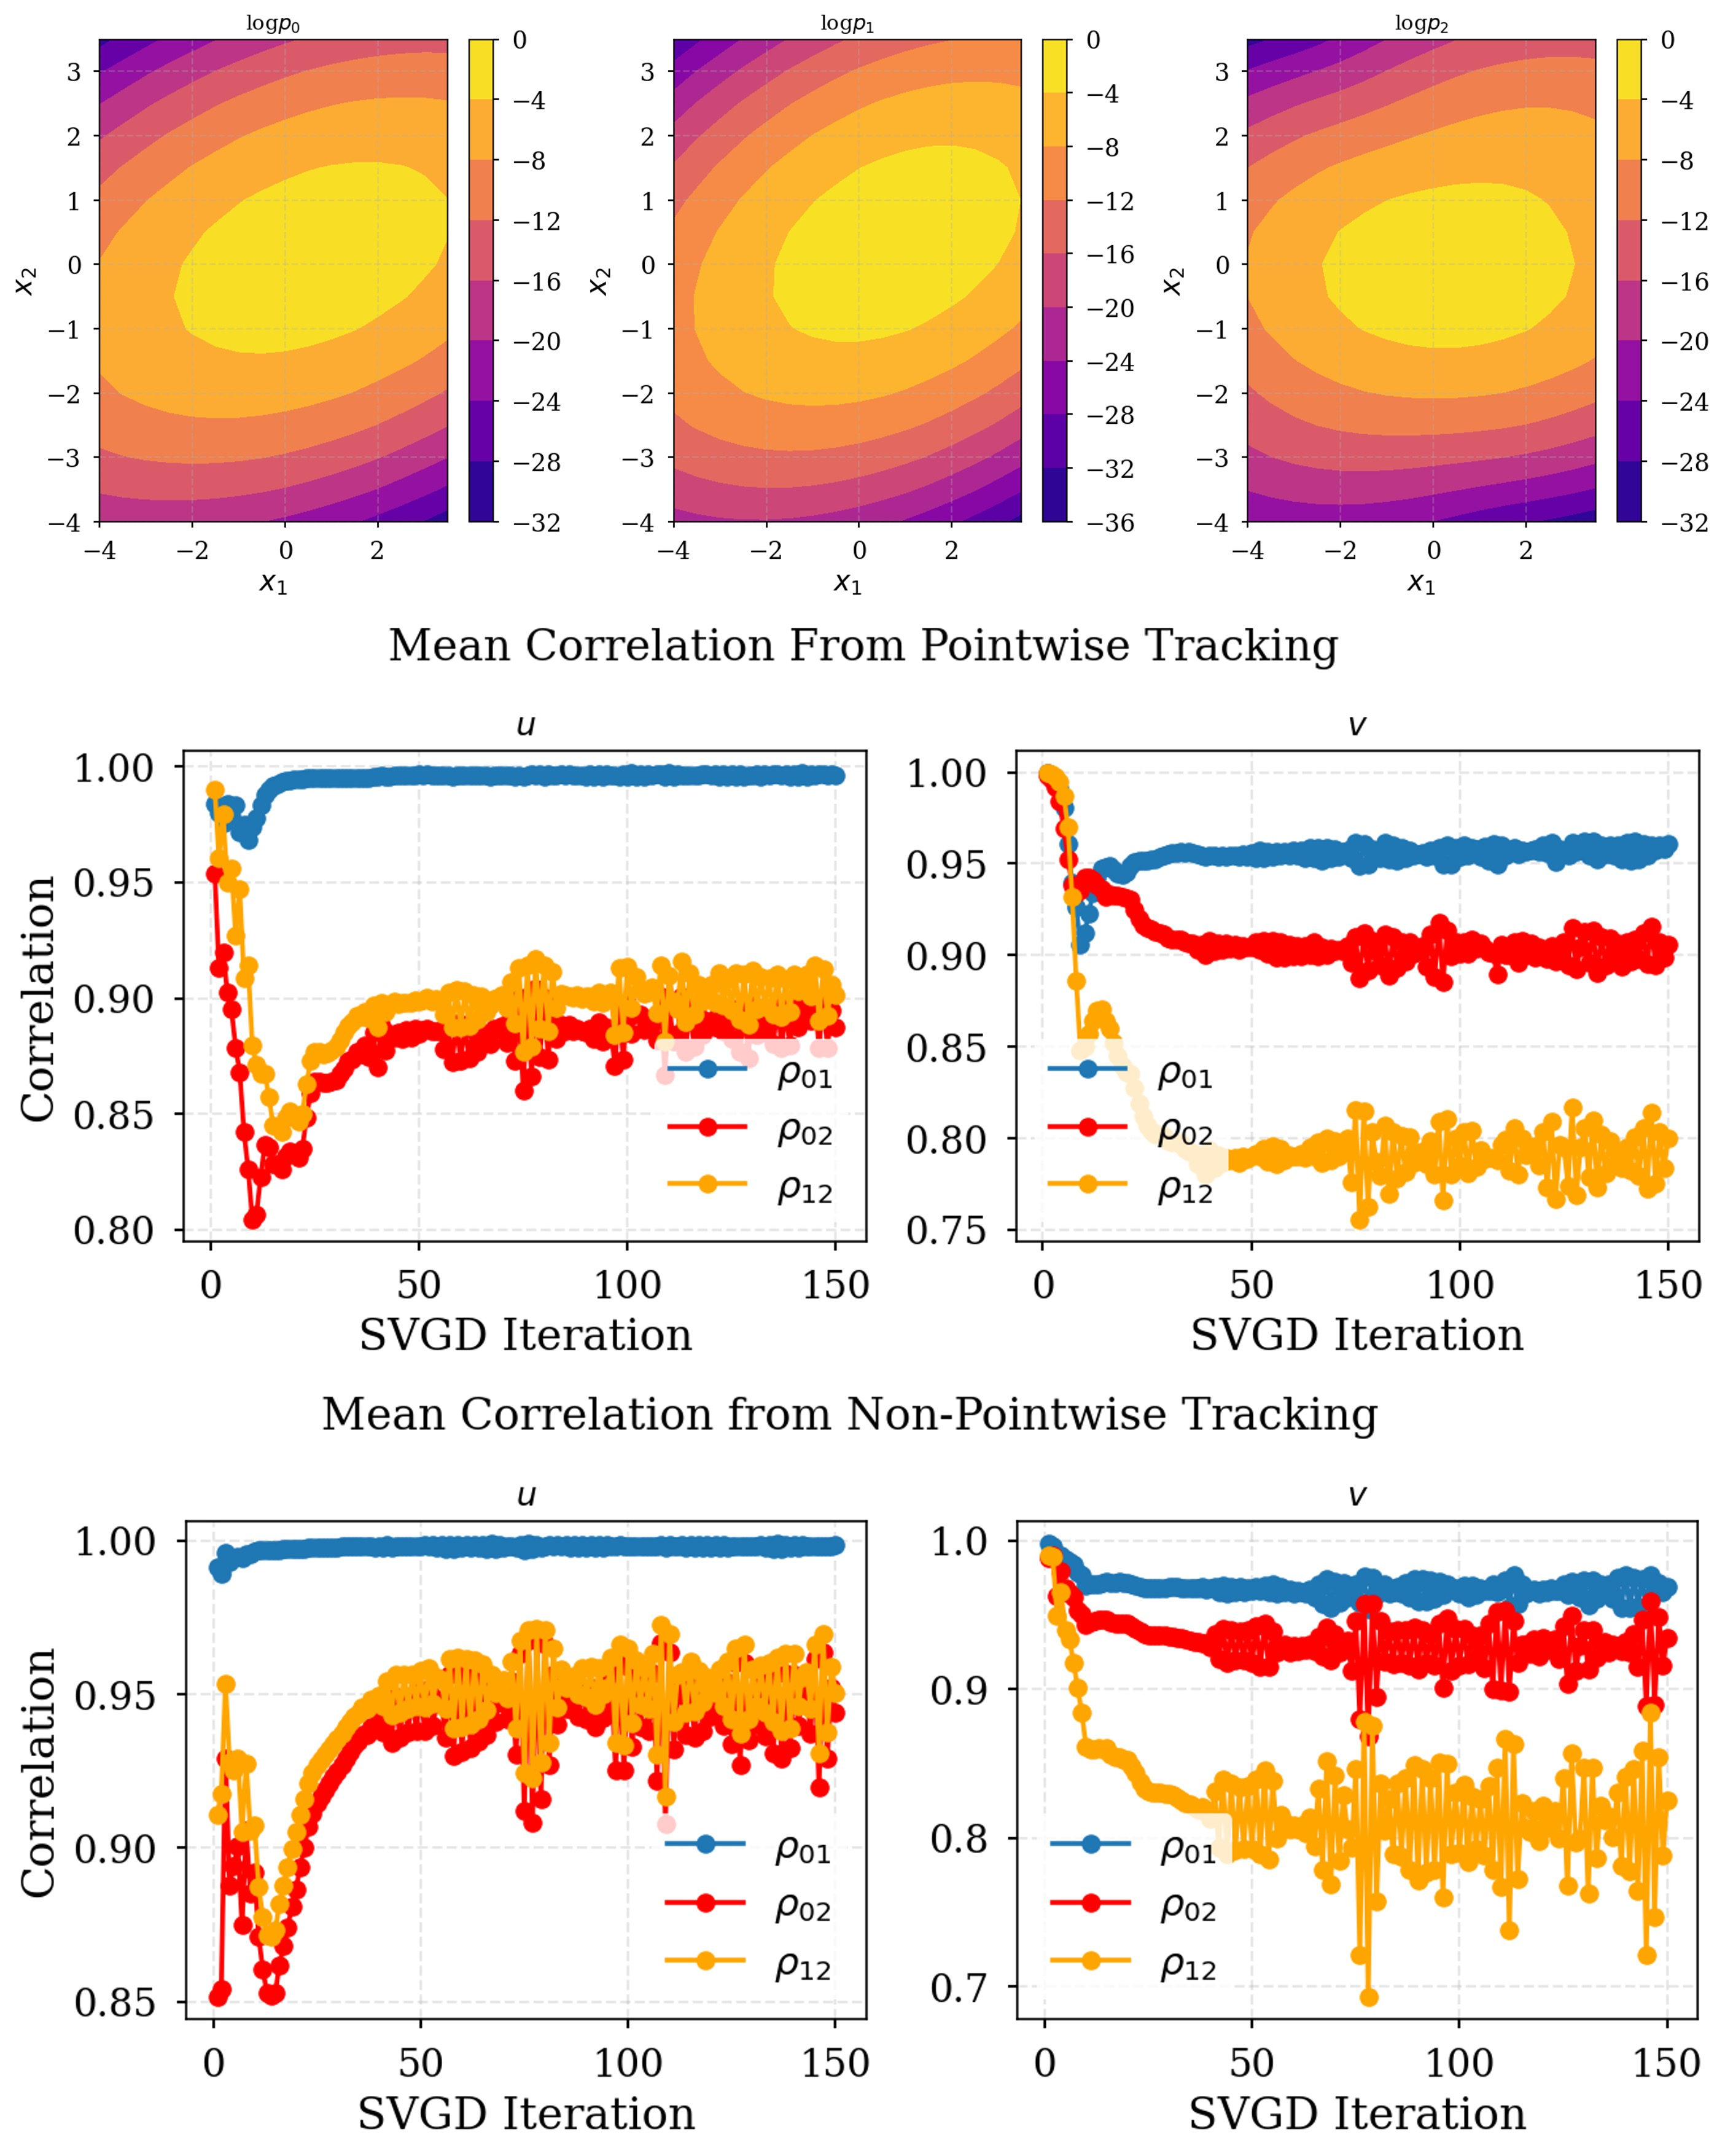
\includegraphics[width=0.8\linewidth]{figures/log_densities_corrs_composite.jpg}
    \caption{Log-densities of each of the model ensemble members (top), followed by sample correlations calculated via \autoref{alg: pilot_sampling_non_adaptive} (middle) and the cumulative approximation for $N_p = 32$}
    \label{fig:svgd_gaussians_pilot_corrs}
\end{figure}


% \textcolor{red}{Online vs offline pilot sampling for correlations. To get correlations avg over all neighbours vs compute for individual neighbours? ACV mean should change based on x particle, though the score remain unchanged for a fixed sample allocation and also rewrite notation $\phi(x)$}



% \begin{equation*}
%     \theta^{(0)}_i \leftarrow \theta^{(0)}_i + \epsilon \phi^{\ast}(\theta^{(0)})
% \end{equation*}

% And similarly, for lower-fidelity models indexed from $1$ to $m$, we can compute the particle positions as:

% \begin{equation*}
%     \theta^{(l)}_i \leftarrow \theta^{(l)}_i + \epsilon \phi^{\ast}(\theta^{(l)}), \quad l=1, \cdots, m
% \end{equation*}

% where

% \begin{align}
%     \phi^{\ast}(\theta^{(0)}) &= \frac{1}{M^{(0)}}\sum_{j=1}^{M^{(0)}}[k(\theta_j, \theta) \grad_{\theta_j}[L_{0} + \log p(\theta_j)] + \grad_{\theta_j} k(\theta_j, \theta)] \\
%     &= \frac{1}{M^{(0)}}\sum_{j=1}^{M^{(0)}}[(k(\theta_j, \theta^{(0)})  + k(\theta_j, \theta^{(1)}) + \cdots + \nonumber\\ 
%     &k(\theta_j, \theta^{(m)})) \grad_{\theta_j}[L_{0} + \log p(\theta_j)]] + \grad_{\theta_j} [k(\theta_j, \theta^{(0)}) + \cdots + k(\theta_j, \theta^{(m)})]\\ \nonumber
% \end{align}

% \begin{align}
%     \phi^{\ast}(\theta^{(l)}) &= \frac{1}{M^{(l)}}\sum_{j=1}^{M^{(l)}}[k(\theta_j, \theta) \grad_{\theta_j}[L_{l} + \log p(\theta_j)] + \grad_{\theta_j} k(\theta_j, \theta)] \\
%     &= \frac{1}{M^{(l)}}\sum_{j=1}^{M^{(l)}}[(k(\theta_j, \theta^{(0)})  + k(\theta_j, \theta^{(1)}) + \cdots + \nonumber \\
%     &k(\theta_j, \theta^{(m)})) \grad_{\theta_j}[L_{l} + \log p(\theta_j)] + \log p(\theta_j)]] + \grad_{\theta_j} k(\theta_j, \theta) \nonumber \\ 
%     &= \frac{1}{M^{(l)}}\sum_{j=1}^{M^{(l)}}[(k(\theta_j, \theta^{(0)})  + k(\theta_j, \theta^{(1)}) + \cdots + \nonumber\\ 
%     &k(\theta_j, \theta^{(m)})) \grad_{\theta_j}[L_{l} + \log p(\theta_j)]] + \grad_{\theta_j} [k(\theta_j, \theta^{(0)}) + \cdots + k(\theta_j, \theta^{(m)})]\\ \nonumber
% \end{align}

% While the $M$ particles are allocated to different models as $M_0, M_1, \cdots, M_m$, the above updates still use all the particles to compute the map at each iteration - this introduces interactions between the multifidelity particles in \stkout{\emph{both} terms of the update: the first term driving the particles to regions of high-probability} \textcolor{red}{(unfortunately, this is not true. When you cut off the kernel matrix to remove the particle interactions amongst the other fidelities, it turns out that only the particle distances corresponding to that fidelity weigh the likelihood)} the second term of the update accounting for the repulsive force that prevents particle collapse into local modes. 
% The repulsive force i.e. the kernel gradient evaluates a shared kernel function over different subsets of $\theta$ in each term, while the force driving particles towards high-probability regions weighs the kernel function by the individual log-likelihoods.
% \textcolor{red}{Interestingly, another algorithmic choice here is the choice of particle positions to use in a given fidelity's updates. For example, if we updated the low-fidelity particle's positions first, these updates could be transmitted to and used by the high fidelity update mechanism in the same step instead of both updates using previously computed positions.}

% The above formulation continues to allow flexibility with regards to the specification and the number of lower-fidelity model; but it also raises additional open questions regarding the following aspects:

% \begin{enumerate}
%     \item The choice of the kernel function for individual model fidelities

%     \item The allocation of particles to different model fidelities (disjoint / overlapping) and how it changes as we step through the method.

%     \item The number and allocation of particles used in computations of the kernel function i.e. neighbourhood selection for particles.

%     \item The frequency of updates to particles of different fidelities, and the update sharing frequency within a single iteration of the outer loop.

%     \item The stopping criterion that assesses convergence to the target distribution.

%     \item Quantitative measurements of discrepancy between distributions fitted via single-fidelity and multiple-fidelity methods.
% \end{enumerate}

% \subsection{KL-Divergence Based Correction with kNN Estimator}





% Perhaps the more pertinent question before we discuss the finer details of the implementation is why we expect this to work at all. Consider the elementary case where we only have access to a single model for likelihood computation. 
% There are two possible bottlenecks: 1. the full data log-likelihood computation is prohibitive on account of the need to process very large-scale data, requiring the modification of standard inference algorithms to handle distributed or streaming data settings 2. the high costs of running the forward model renders the inference intractable without resorting to surrogate approximations. 

% A prominent line of work that deals with the first case uses the so-called `consensus Monte Carlo methods' \citep{rabinovich_variational_2015,scott_bayes_2016}. Here a data sharding (partitioning) step is followed by independent posterior sampling on multiple machines conditioned on the data partitions. 
% The communication overhead is avoided by combining the posterior draws to form a `consensus' belief about the model unknowns.
% The algorithm is exact for Gaussian posteriors, but has been found to be broadly useful for non-Gaussian settings too.

% Rather than modifying the inference algorithm, practitioners have recently focused on exploiting redundancies in the dataset by identifying a weighted subset of the data known as the \emph{coreset}, that originated in computational geometry \citep{agarwal_geometric_2007} and later found popularity in scalable clustering methods.
% Discussions on Bayesian coreset methods \citep{huggins_coresets_2016,campbell_automated_2019} focus on high-probability guarantees for the approximation quality of the resulting log-likelihood and demonstrate their superior performance over random subsampling methods. A superficial analogy we can draw is the treatment of the high-fidelity particles as our coreset, and the kernel function that accounts for all model fidelities as a means to enforce a weighted log-likelihood.

% Akin to coresets, the concept of `graph coarsening' is ubiquitous all across scientific computing and machine learning methods for graph representation \citep{chen_graph_2022}. The goal of graph coarsening is to uncover a smaller graph that faithfully reflects the structure of the original graph. The coarse graph/s is/are typically determined using notions of pairwise similarity, algebraic distance, independent sets, sketching based on leverage scores and other criteria. 
% In this framework, we can treat the selection of high-fidelity particles as a form of graph coarsening, if the features for these particles are constructed from aggregation of lower-fidelity particles rather than assignment of existing particles.

% While these techniques do not directly relate to the workings or performance of our proposed method relying on the non-parametric version of the SVGD method, they serve as useful guiding principles to improve practical implementations which typically rely on random particle subsampling for efficient kernel computations. 

% A simpler analogy arises from the purview of dynamical systems: the asymptotic behaviour of SVGD is characterized by the Vlasov equation \citep{liu_stein_2017}. 
% Then, deploying a multistep predictor-corrector method to solve the resulting ordinary differential equation would be akin to performing a sequence of low-fidelity predictions for particle positions to serve as the initial guess, followed by a correction step for some or all particles via the high-fidelity likelihood i.e. the fidelity assignment \emph{alternates} rather than preceding or following the model updates .
% The benefits of such an approach would be practically realized when the equivalent cost in terms of single-fidelity evaluations is measurably brought down in implementations. 
% However, determination of `when to correct, what to correct' is also a non-trivial problem.

% In the following sections, we will lay out a framework to evaluate some of these key choices and provide more details of our proposed method.

% \subsection{Particle assignment to various fidelities}

% \emph{Method 0: Non-randomized Assignment}
% The simplest possible setting does not attempt to reassign particles, instead, at every iteration, a fixed proportion of the particles is treated as the lower-fidelity likelihood update while the remaining are high-fidelity updates. 
% We look at the number of iterations required for convergence by monitoring the hyperparameters of the kernel function.

% \noindent \emph{Method 1: Randomized Assignment}
% To correct for possible bias due to incorrect particle assignment, randomized assignment shuffles the particles between the different fidelities after one or more update steps.

% \noindent \emph{Method 2: Assignment based on clustering methods}
% For the first time, we consider the setting where a small subset of particles is deemed to be non-redundant and a summarization of the dataset. Here, we incorporate a clustering-based heuristic that determines the high-fidelity particles based on a suitable measure of distance.
% It is of particular importance to ensure that the cost of pairwise distance computations does not grow or outweigh the cost of simpler methods such as randomized assignment i.e. there is possibility of reuse for these when we actually perform the Stein updates.


% \noindent \emph{Method 3: Resource allocation using model correlations}

% \subsection{Graph Network Based Propagation}
% Deep learning methods that model arbitrary relational structures between elements, such as graph networks (GNs), are surveyed in \cite{battaglia_relational_2018}. 

% GNs model a domain by decomposing it into a graphical representation $\CG=\{\CV, \CE\}$ - nodes $\CV$ that represent individual features and edges $\CE$ that describe directed or undirected interactions between nodes. 
% The learning proceeds by first defining a neighbourhood for individual nodes. This is followed by a message-passing block that updates node features based on aggregating interactions with all or a subset of its possible neighbours. Chaining several such blocks with intermediate nonlinear activations results in a GN which accepts an arbitrarily sized graph as input and returns either a transformed graph or some global property of the graph as the output. 

% Superficially translating the graphical representation to a particle-based updates / normalizing flow setup suggests the propagation of augmented node features $[x, \log p(x)]$ where both the particle positions $x$ and their log-likelihoods $\log p(x)$ are updated as they pass through the message-passing blocks. Two key advantages offered by graph-based methods are their inherent invariance to permutations (unlike MLPs) and their ability to operate on graphs of arbitrary sizes without modifications to the architecture. 
% This feature translates to so-called `discretization invariance' in expressive methods for learning PDEs such as neural operators \citep{Li2020} which exhibit good generalization properties even when trained on low-resolution data. GNs have been successfully used to simulate complex physics with long rollout times, e.g. \cite{sanchez-gonzalez_learning_2020}.

% Without additional constraints however, a GN is not directly compatible with the workflow of particle-based methods for inference, where the key goal is to constrain the transport of individual particles by minimizing a particular discrepancy function that characterizes the quality of the posterior approximation. 
% It is also unclear if the discretization-invariance property grants any advantages in better representation of the posterior density in low-data settings. 
% However, the advances in scaling GNs to very large graphs with millions of nodes suggest opportunities to influence the development of scalable particle methods for inference and offer a more flexible workflow. 
% We begin with a brief overview of our proposed changes below:

% \subsection{Particle Swarm Optimization based methods}
% (with a specific interest in multi-population cooperative particle swarm optimization, even though we are not specifically targeting optimization) - see \url{https://ieeexplore.ieee.org/document/9967774} for an example.


% \subsection{Sparse Kernel Updates}

\section{Results}

\subsection{Multivariate Gaussian Model Problem}

To demonstrate the working of the algorithm, we use a simple benchmark problem where the target densities are multivariate Gaussians $\{p_i(x)\}_{i=0}^{M-1}$, with $M=3$, and each $p_i$ parametrized by its respective mean and covariance $(\mu_i, \Sigma_i)$:

The associated cost vector is given by $w=\{10^{-m}\}_{m=0}^{M-1}$.




\subsection{Estimator Performance for Monte-Carlo Integration}

\subsection{Bayesian Inference}

% \subsection{Optimal Experimental Design via MF-SVGD Bayesian Inference}


% \subsection{Generalizing Compressed Representations to Higher Particle Counts}
% We consider the case where the original inference is performed on a small set of $N$ particles, but density estimation may be desired with additional particles at test time. 
% Then we need the ability to perform rapid approximation of positions for $K$ new particles introduced at test time. 
% This would require $\Mycomb[(N+K)]{2} - \Mycomb[N]{2} = \frac{1}{2}(K^2 + 2NK - K)$ additional distance calculations and $K$ potentially expensive likelihood computations followed by density estimation in the naive setting. 
% By contrast, a trained parametric simulator that 1. is `discretization invariant' in some sense by capturing the key relationships between existing particles 2. can allocate a large fraction of particles to one or more lower-fidelity models can rapidly convert these to high-quality posterior samples.

\subsection{}

\section{Conclusions and Extensions}

In this work, we considered the application of multifidelity surrogate and multifidelity estimator techniques to a general-purpose non-parametric variational inference technique, namely Stein Variational Gradient Descent (SVGD). SVGD has numerous applications, including hypothesis testing, development of traditional CVs for MCMC, and  Bayesian inference for neural networks - settings with access to a smooth and differentiable posterior density. 

We proposed two alternate estimators that take advantage of lower-fidelity forward models to accomodate a larger number of particles propagating to the target density. The first estimator is based on a simple idea from additive-correction based multi-fidelity surrogates, where a lower-fidelity gradient estimate is corrected through a score ratio computed on a smaller subset of particles. Randomization of this subset at every SVGD iteration eventually drives the particle system to a better approximation of the high-fidelity target density; however the distribution of particles is problem-specific and based on empirical comparisons to the vanilla SVGD update. 
The second estimator draws on well-established theory from approximate control variate (ACV)-based estimators - using the cost and correlation estimates between parts of the gradient term, we learn the control variate weights and a sample allocation strategy to distribute particles amongst various fidelities under different computational budget scenarios. 

We explored the benefits of these estimators for Monte-Carlo integration with different test functions compared to traditional Monte-Carlo methods and computations under vanilla SVGD.

\appendix
% \section{An example appendix} 
% \lipsum[71]



\section*{Acknowledgments}
This work is supported in part by the National Science Foundation Graduate Research Fellowship under Grant No. DGE 1841052, the Department of Navy award N00014-23-1-2735 issued by the Office of Naval Research, and through computational resources and services provided by Advanced Research Computing at the University of Michigan, Ann Arbor.


\bibliographystyle{siamplain}
\bibliography{local,references}

\end{document}

